\documentclass[dvipdfmx]{jsarticle}
\setcounter{section}{2}
\setcounter{subsection}{5}
\usepackage{xr}
\externaldocument{2.2.3}
\externaldocument{2.2.4}
\externaldocument{2.2.5}
\usepackage{amsmath,amsfonts,amssymb,array,comment,mathtools,url,docmute}
\usepackage{longtable,booktabs,dcolumn,tabularx,mathtools,multirow,colortbl,xcolor}
\usepackage[dvipdfmx]{graphics}
\usepackage{bmpsize}
\usepackage{amsthm}
\usepackage{enumitem}
\setlistdepth{20}
\renewlist{itemize}{itemize}{20}
\setlist[itemize]{label=•}
\renewlist{enumerate}{enumerate}{20}
\setlist[enumerate]{label=\arabic*.}
\setcounter{MaxMatrixCols}{20}
\setcounter{tocdepth}{3}
\newcommand{\rotin}{\text{\rotatebox[origin=c]{90}{$\in $}}}
\newcommand{\amap}[6]{\text{\raisebox{-0.7cm}{\begin{tikzpicture} 
  \node (a) at (0, 1) {$\textstyle{#2}$};
  \node (b) at (#6, 1) {$\textstyle{#3}$};
  \node (c) at (0, 0) {$\textstyle{#4}$};
  \node (d) at (#6, 0) {$\textstyle{#5}$};
  \node (x) at (0, 0.5) {$\rotin $};
  \node (x) at (#6, 0.5) {$\rotin $};
  \draw[->] (a) to node[xshift=0pt, yshift=7pt] {$\textstyle{\scriptstyle{#1}}$} (b);
  \draw[|->] (c) to node[xshift=0pt, yshift=7pt] {$\textstyle{\scriptstyle{#1}}$} (d);
\end{tikzpicture}}}}
\newcommand{\twomaps}[9]{\text{\raisebox{-0.7cm}{\begin{tikzpicture} 
  \node (a) at (0, 1) {$\textstyle{#3}$};
  \node (b) at (#9, 1) {$\textstyle{#4}$};
  \node (c) at (#9+#9, 1) {$\textstyle{#5}$};
  \node (d) at (0, 0) {$\textstyle{#6}$};
  \node (e) at (#9, 0) {$\textstyle{#7}$};
  \node (f) at (#9+#9, 0) {$\textstyle{#8}$};
  \node (x) at (0, 0.5) {$\rotin $};
  \node (x) at (#9, 0.5) {$\rotin $};
  \node (x) at (#9+#9, 0.5) {$\rotin $};
  \draw[->] (a) to node[xshift=0pt, yshift=7pt] {$\textstyle{\scriptstyle{#1}}$} (b);
  \draw[|->] (d) to node[xshift=0pt, yshift=7pt] {$\textstyle{\scriptstyle{#2}}$} (e);
  \draw[->] (b) to node[xshift=0pt, yshift=7pt] {$\textstyle{\scriptstyle{#1}}$} (c);
  \draw[|->] (e) to node[xshift=0pt, yshift=7pt] {$\textstyle{\scriptstyle{#2}}$} (f);
\end{tikzpicture}}}}
\renewcommand{\thesection}{第\arabic{section}部}
\renewcommand{\thesubsection}{\arabic{section}.\arabic{subsection}}
\renewcommand{\thesubsubsection}{\arabic{section}.\arabic{subsection}.\arabic{subsubsection}}
\everymath{\displaystyle}
\allowdisplaybreaks[4]
\usepackage{vtable}
\theoremstyle{definition}
\newtheorem{thm}{定理}[subsection]
\newtheorem*{thm*}{定理}
\newtheorem{dfn}{定義}[subsection]
\newtheorem*{dfn*}{定義}
\newtheorem{axs}[dfn]{公理}
\newtheorem*{axs*}{公理}
\renewcommand{\headfont}{\bfseries}
\makeatletter
  \renewcommand{\section}{%
    \@startsection{section}{1}{\z@}%
    {\Cvs}{\Cvs}%
    {\normalfont\huge\headfont\raggedright}}
\makeatother
\makeatletter
  \renewcommand{\subsection}{%
    \@startsection{subsection}{2}{\z@}%
    {0.5\Cvs}{0.5\Cvs}%
    {\normalfont\LARGE\headfont\raggedright}}
\makeatother
\makeatletter
  \renewcommand{\subsubsection}{%
    \@startsection{subsubsection}{3}{\z@}%
    {0.4\Cvs}{0.4\Cvs}%
    {\normalfont\Large\headfont\raggedright}}
\makeatother
\makeatletter
\renewenvironment{proof}[1][\proofname]{\par
  \pushQED{\qed}%
  \normalfont \topsep6\p@\@plus6\p@\relax
  \trivlist
  \item\relax
  {
  #1\@addpunct{.}}\hspace\labelsep\ignorespaces
}{%
  \popQED\endtrivlist\@endpefalse
}
\makeatother
\renewcommand{\proofname}{\textbf{証明}}
\usepackage{tikz,graphics}
\usepackage[dvipdfmx]{hyperref}
\usepackage{pxjahyper}
\hypersetup{
 setpagesize=false,
 bookmarks=true,
 bookmarksdepth=tocdepth,
 bookmarksnumbered=true,
 colorlinks=false,
 pdftitle={},
 pdfsubject={},
 pdfauthor={},
 pdfkeywords={}}
\begin{document}
%\hypertarget{jordanux6a19ux6e96ux5f62}{%
\subsection{Jordan標準形}%\label{jordanux6a19ux6e96ux5f62}}
%\hypertarget{jordanux6a19ux6e96ux5f62-1}{%
\subsubsection{Jordan標準形}%\label{jordanux6a19ux6e96ux5f62-1}}
\begin{dfn*}[定義\ref{Jordan細胞の定義}の再掲]
体$K$の元$k$を用いて$A_{nn} \in M_{nn}(K)$なる行列$A_{nn}$が次式のように表されるとき、その行列$A_{nn}$をその元$k$のJordan細胞、$k$細胞などといい$J(k,n)$と書く。
\begin{align*}
A_{nn} = \begin{pmatrix}
k & 1 & \  & \  & O \\
\  & k & 1 & \  & \  \\
\  & \  & k & \ddots & \  \\
\  & \  & \  & \ddots & 1 \\
O & \  & \  & \  & k \\
\end{pmatrix}
\end{align*}
\end{dfn*}
\begin{thm}\label{2.2.6.1}
代数的閉体$K$上の$n$次元vector空間$V$における線形写像$f:V \rightarrow V$の固有多項式$\varPhi_{f}$が互いに異なるその体$K$の元々$\lambda_{i}$を用いて$\sum_{i \in \varLambda_{s}} n_{i} = n$として次式のように表されることができるので、そうするとき、次のことが成り立つ。
\begin{align*}
\varPhi_{f} = \prod_{i \in \varLambda_{s}} \left( X - \lambda_{i} \right)^{n_{i}}
\end{align*}
\begin{itemize}
\item
  $\forall i \in \varLambda_{s}$に対し、線形写像$\lambda_{i}I_{V} - f$は核$\ker\left( \lambda_{i}I_{V} - f \right)^{n_{i}}$における冪零変換である。
\item
  $\forall i \in \varLambda_{s}$に対し、その核$\ker\left( \lambda_{i}I_{V} - f \right)^{n_{i}}$は$f$-不変である。
\item
  $\forall i \in \varLambda_{s}$に対し、その核$\ker\left( \lambda_{i}I_{V} - f \right)^{n_{i}}$における冪零変換$\lambda_{i}I_{V} - f$の不変系$Q_{i}$が$Q_{i} = \left( q_{ij} \right)_{j \in \varLambda_{r_{i}}}$と与えられたらば、その核$\ker\left( \lambda_{i}I_{V} - f \right)^{n_{i}}$の次式のようなある基底$\mathcal{B}_{i}$が存在して、
\begin{align*}
\mathcal{B}_{i} = \left\langle \begin{matrix}
\mathbf{v}_{i1} & \mathbf{v}_{i2} & \cdots & \mathbf{v}_{ir_{i}} \\
\left( f - \lambda_{i}I_{V} \right)\left( \mathbf{v}_{i1} \right) & \left( f - \lambda_{i}I_{V} \right)\left( \mathbf{v}_{i2} \right) & \cdots & \left( f - \lambda_{i}I_{V} \right)\left( \mathbf{v}_{ir_{i}} \right) \\
 \vdots & \vdots & \ddots & \vdots \\
\left( f - \lambda_{i}I_{V} \right)^{q_{i1} - 1}\left( \mathbf{v}_{i1} \right) & \left( f - \lambda_{i}I_{V} \right)^{q_{i2} - 1}\left( \mathbf{v}_{i2} \right) & \cdots & \left( f - \lambda_{i}I_{V} \right)^{q_{ir_{i}} - 1}\left( \mathbf{v}_{ir_{i}} \right) \\
\end{matrix} \right\rangle
\end{align*}
これに関する線形写像$f|\ker\left( \lambda_{i}I_{V} - f \right)^{n_{i}}$の表現行列$\left[ f|\ker\left( \lambda_{i}I_{V} - f \right)^{n_{i}} \right]_{\mathcal{B}_{i}}^{\mathcal{B}_{i}}$が次式のように一意的に表されることができる。
\begin{align*}
\left[ f|\ker\left( \lambda_{i}I_{V} - f \right)^{n_{i}} \right]_{\mathcal{B}_{i}}^{\mathcal{B}_{i}} = \begin{pmatrix}
J\left( \lambda_{i},q_{i1} \right) & \  & \  & O \\
\  & J\left( \lambda_{i},q_{i2} \right) & \  & \  \\
\  & \  & \ddots & \  \\
O & \  & \  & J\left( \lambda_{i},q_{ir_{i}} \right) \\
\end{pmatrix}
\end{align*}
\end{itemize}
\end{thm}
\begin{dfn}\label{Jordan block}
このときの固有値$\lambda_{i}$に対する表現行列$\left[ f|\ker\left( \lambda_{i}I_{V} - f \right)^{n_{i}} \right]_{\mathcal{B}_{i}}^{\mathcal{B}_{i}}$をその固有値$\lambda_{i}$に対するJordan block、Jordan塊といい、ここでは、$J\left( \lambda_{i};Q_{i} \right)$と書くことにする。
\end{dfn}
\begin{proof}
代数的閉体$K$上の$n$次元vector空間$V$における線形写像$f:V \rightarrow V$の固有多項式$\varPhi_{f}$が互いに異なるその体$K$の元々$\lambda_{i}$を用いて$\sum_{i \in \varLambda_{s}} n_{i} = n$として次式のように表されることができるので、そうするとき、
\begin{align*}
\varPhi_{f} = \prod_{i \in \varLambda_{s}} \left( X - \lambda_{i} \right)^{n_{i}}
\end{align*}
$\forall i \in \varLambda_{s}\forall\mathbf{v} \in \ker\left( \lambda_{i}I_{V} - f \right)^{n_{i}}$に対し、$\left( \lambda_{i}I_{V} - f \right)^{n_{i}}\left( \mathbf{v} \right) = \mathbf{0}$が成り立つので、線形写像$\lambda_{i}I_{V} - f$は核$\ker\left( \lambda_{i}I_{V} - f \right)^{n_{i}}$における冪零変換である。\par
さらに、$\forall i \in \varLambda_{s}\forall\mathbf{v} \in \ker\left( \lambda_{i}I_{V} - f \right)^{n_{i}}$に対し、定理\ref{2.2.3.5}より次のようになることから、
\begin{align*}
\left( \lambda_{i}I_{V} - f \right)^{n_{i}}\left( f\left( \mathbf{v} \right) \right) &= \left( \lambda_{i}I_{V} - f \right)^{n_{i}} \circ f\left( \mathbf{v} \right)\\
&= f \circ \left( \lambda_{i}I_{V} - f \right)^{n_{i}}\left( \mathbf{v} \right)\\
&= f\left( \left( \lambda_{i}I_{V} - f \right)^{n_{i}}\left( \mathbf{v} \right) \right)\\
&= f\left( \mathbf{0} \right) = \mathbf{0}
\end{align*}
$f\left( \mathbf{v} \right) \in \ker\left( \lambda_{i}I_{V} - f \right)^{n_{i}}$が成り立ち、したがって、その核$\ker\left( \lambda_{i}I_{V} - f \right)^{n_{i}}$は$f$-不変である。\par
$\forall i \in \varLambda_{s}$に対し、その核$\ker\left( \lambda_{i}I_{V} - f \right)^{n_{i}}$における冪零変換$\lambda_{i}I_{V} - f$の不変系$Q_{i}$が$Q_{i} = \left( q_{ij} \right)_{j \in \varLambda_{r_{i}}}$と与えられたらば、分解定理よりその核$\ker\left( \lambda_{i}I_{V} - f \right)^{n_{i}}$の次元はその自然数$n_{i}$に等しく、定理\ref{2.2.5.3}より次式のような$n_{i}$つのvectorsの組$\mathcal{C}_{i}$はその核$\ker\left( \lambda_{i}I_{V} - f \right)^{n_{i}}$の基底をなす。
\begin{align*}
\mathcal{C}_{i} = \left\langle \begin{matrix}
\mathbf{v}_{i1} & \mathbf{v}_{i2} & \cdots & \mathbf{v}_{ir_{i}} \\
\left( \lambda_{i}I_{V} - f \right)\left( \mathbf{v}_{i1} \right) & \left( \lambda_{i}I_{V} - f \right)\left( \mathbf{v}_{i2} \right) & \cdots & \left( \lambda_{i}I_{V} - f \right)\left( \mathbf{v}_{ir_{i}} \right) \\
 \vdots & \vdots & \ddots & \vdots \\
\left( \lambda_{i}I_{V} - f \right)^{q_{i1} - 1}\left( \mathbf{v}_{i1} \right) & \left( \lambda_{i}I_{V} - f \right)^{q_{i2} - 1}\left( \mathbf{v}_{i2} \right) & \cdots & \left( \lambda_{i}I_{V} - f \right)^{q_{ir_{i}} - 1}\left( \mathbf{v}_{ir_{i}} \right) \\
\end{matrix} \right\rangle
\end{align*}
このとき、線形写像$f - \lambda_{i}I_{V}$も定理\ref{2.2.5.3}、定理\ref{2.2.5.6}より不変系$Q_{i}$のその核$\ker\left( \lambda_{i}I_{V} - f \right)^{n_{i}}$における冪零変換でもあるので、定理\ref{2.2.5.9}より次式のようなある基底$\mathcal{B}_{i}$が存在して、
\begin{align*}
\mathcal{B}_{i} = \left\langle \begin{matrix}
\mathbf{v}_{i1} & \mathbf{v}_{i2} & \cdots & \mathbf{v}_{ir_{i}} \\
\left( f - \lambda_{i}I_{V} \right)\left( \mathbf{v}_{i1} \right) & \left( f - \lambda_{i}I_{V} \right)\left( \mathbf{v}_{i2} \right) & \cdots & \left( f - \lambda_{i}I_{V} \right)\left( \mathbf{v}_{ir_{i}} \right) \\
 \vdots & \vdots & \ddots & \vdots \\
\left( f - \lambda_{i}I_{V} \right)^{q_{i1} - 1}\left( \mathbf{v}_{i1} \right) & \left( f - \lambda_{i}I_{V} \right)^{q_{i2} - 1}\left( \mathbf{v}_{i2} \right) & \cdots & \left( f - \lambda_{i}I_{V} \right)^{q_{ir_{i}} - 1}\left( \mathbf{v}_{ir_{i}} \right) \\
\end{matrix} \right\rangle
\end{align*}
これに関するその冪零変換$f - \lambda_{i}I_{V}$の表現行列$\left[ f - \lambda_{i}I_{V} \right]_{\mathcal{B}_{i}}^{\mathcal{B}_{i}}$が次式のように表されることができる。
\begin{align*}
\left[ f - \lambda_{i}I_{V} \right]_{\mathcal{B}_{i}}^{\mathcal{B}_{i}} = \begin{pmatrix}
J\left( 0,q_{i1} \right) & \  & \  & O \\
\  & J\left( 0,q_{i2} \right) & \  & \  \\
\  & \  & \ddots & \  \\
O & \  & \  & J\left( 0,q_{ir_{i}} \right) \\
\end{pmatrix}
\end{align*}
これにより、$q$次単位行列$I_{q}$を用いて次のようになる。
\begin{align*}
\left[ f|\ker\left( \lambda_{i}I_{V} - f \right)^{n_{i}} \right]_{\mathcal{B}_{i}}^{\mathcal{B}_{i}} &= [ f]_{\mathcal{B}_{i}}^{\mathcal{B}_{i}} - \left[ \lambda_{i}I_{V} \right]_{\mathcal{B}_{i}}^{\mathcal{B}_{i}} + \left[ \lambda_{i}I_{V} \right]_{\mathcal{B}_{i}}^{\mathcal{B}_{i}}\\
&= \left[ f - \lambda_{i}I_{V} \right]_{\mathcal{B}_{i}}^{\mathcal{B}_{i}} + \lambda_{i}\left[ I_{V} \right]_{\mathcal{B}_{i}}^{\mathcal{B}_{i}}\\
&= \begin{pmatrix}
J\left( 0,q_{i1} \right) & \  & \  & O \\
\  & J\left( 0,q_{i2} \right) & \  & \  \\
\  & \  & \ddots & \  \\
O & \  & \  & J\left( 0,q_{ir_{i}} \right) \\
\end{pmatrix} + \lambda_{i}\begin{pmatrix}
I_{q_{i1}} & \  & \  & O \\
\  & I_{q_{i2}} & \  & \  \\
\  & \  & \ddots & \  \\
O & \  & \  & I_{ir_{i}} \\
\end{pmatrix}\\
&= \begin{pmatrix}
J\left( 0,q_{i1} \right) + \lambda_{i}I_{q_{i1}} & \  & \  & O \\
\  & J\left( 0,q_{i2} \right) + \lambda_{i}I_{q_{i2}} & \  & \  \\
\  & \  & \ddots & \  \\
O & \  & \  & J\left( 0,q_{ir_{i}} \right) + \lambda_{i}I_{q_{ir_{1}}} \\
\end{pmatrix}\\
&= \begin{pmatrix}
J\left( \lambda_{i},q_{i1} \right) & \  & \  & O \\
\  & J\left( \lambda_{i},q_{i2} \right) & \  & \  \\
\  & \  & \ddots & \  \\
O & \  & \  & J\left( \lambda_{i},q_{ir_{i}} \right) \\
\end{pmatrix}
\end{align*}\par
このとき、その固有値$\lambda_{i}$に対し、冪零変換$\lambda_{i}I_{V} - f$が一意的に存在し、定理\ref{2.2.5.6}より冪零変換$\lambda_{i}I_{V} - f$の不変系が$Q_{i}$と一意的に与えられるので、その基底$\mathcal{B}_{i}$に関する線形写像$f|\ker\left( \lambda_{i}I_{V} - f \right)^{n_{i}}$の上記の形の表現行列$\left[ f|\ker\left( \lambda_{i}I_{V} - f \right)^{n_{i}} \right]_{\mathcal{B}_{i}}^{\mathcal{B}_{i}}$が一意的に表されることができる。
\end{proof}
\begin{thm}\label{2.2.6.2}
代数的閉体$K$上の$n$次元vector空間$V$における線形写像$f:V \rightarrow V$の固有多項式$\varPhi_{f}$が互いに異なるその体$K$の元々$\lambda_{i}$を用いて$\sum_{i \in \varLambda_{s}} n_{i} = n$として次式のように表されることができるので、そうするとき、
\begin{align*}
\varPhi_{f} = \prod_{i \in \varLambda_{s}} \left( X - \lambda_{i} \right)^{n_{i}}
\end{align*}
$\forall i \in \varLambda_{s}$に対し、定理\ref{2.2.6.1}
よりその核$\ker\left( \lambda_{i}I_{V} - f \right)^{n_{i}}$における冪零変換$\lambda_{i}I_{V} - f$の不変系$Q_{i}$が$Q_{i} = \left( q_{ij} \right)_{j \in \varLambda_{r_{i}}}$と与えられたらば、そのvector空間$V$の次式のようなある基底$\left\langle \mathcal{B}_{i} \right\rangle_{i \in \varLambda_{s}}$が存在して、
\begin{align*}
\mathcal{B}_{i} = \left\langle \begin{matrix}
\mathbf{v}_{i1} & \mathbf{v}_{i2} & \cdots & \mathbf{v}_{ir_{i}} \\
\left( f - \lambda_{i}I_{V} \right)\left( \mathbf{v}_{i1} \right) & \left( f - \lambda_{i}I_{V} \right)\left( \mathbf{v}_{i2} \right) & \cdots & \left( f - \lambda_{i}I_{V} \right)\left( \mathbf{v}_{ir_{i}} \right) \\
 \vdots & \vdots & \ddots & \vdots \\
\left( f - \lambda_{i}I_{V} \right)^{q_{i1} - 1}\left( \mathbf{v}_{i1} \right) & \left( f - \lambda_{i}I_{V} \right)^{q_{i2} - 1}\left( \mathbf{v}_{i2} \right) & \cdots & \left( f - \lambda_{i}I_{V} \right)^{q_{ir_{i}} - 1}\left( \mathbf{v}_{ir_{i}} \right) \\
\end{matrix} \right\rangle
\end{align*}
これが$\mathcal{B}$とおかれると、これに関する線形写像$f$の表現行列$[ f]_{\mathcal{B}}^{\mathcal{B}}$が次式のように表されることができる。
\begin{align*}
[ f]_{\mathcal{B}}^{\mathcal{B}} = \begin{pmatrix}
J\left( \lambda_{1};Q_{1} \right) & \  & \  & O \\
\  & J\left( \lambda_{2};Q_{2} \right) & \  & \  \\
\  & \  & \ddots & \  \\
O & \  & \  & J\left( \lambda_{s};Q_{s} \right) \\
\end{pmatrix}
\end{align*}
しかも、その表現行列$[ f]_{\mathcal{B}}^{\mathcal{B}}$の中に含まれるJordan塊たちの順序を除けば、その表現行列$[ f]_{\mathcal{B}}^{\mathcal{B}}$はその線形写像$f$に対し一意的に決まる。
\end{thm}
\begin{dfn}
このときの線形写像$f$に対する表現行列$[ f]_{\mathcal{B}}^{\mathcal{B}}$をJordan標準形といい、このような形の行列をJordan行列、この基底$\mathcal{B}$をJordan基底という。
\end{dfn}
\begin{proof}
代数的閉体$K$上の$n$次元vector空間$V$における線形写像$f:V \rightarrow V$の固有多項式$\varPhi_{f}$が互いに異なるその体$K$の元々$\lambda_{i}$を用いて$\sum_{i \in \varLambda_{s}} n_{i} = n$として次式のように表されることができるので、そうするとき、
\begin{align*}
\varPhi_{f} = \prod_{i \in \varLambda_{s}} \left( X - \lambda_{i} \right)^{n_{i}}
\end{align*}
$\forall i \in \varLambda_{s}$に対し、定理\ref{2.2.6.1}よりその核$\ker\left( \lambda_{i}I_{V} - f \right)^{n_{i}}$における冪零変換$\lambda_{i}I_{V} - f$の不変系$Q_{i}$が$Q_{i} = \left( q_{ij} \right)_{j \in \varLambda_{r_{i}}}$と与えられたらば、その核$\ker\left( \lambda_{i}I_{V} - f \right)^{n_{i}}$のある基底$\mathcal{B}_{i}$が存在してこれに関する線形写像$f|\ker\left( \lambda_{i}I_{V} - f \right)^{n_{i}}$の表現行列$\left[ f|\ker\left( \lambda_{i}I_{V} - f \right)^{n_{i}} \right]_{\mathcal{B}_{i}}^{\mathcal{B}_{i}}$が次式のように表されることができる。
\begin{align*}
\left[ f|\ker\left( \lambda_{i}I_{V} - f \right)^{n_{i}} \right]_{\mathcal{B}_{i}}^{\mathcal{B}_{i}} = J\left( \lambda_{i};Q_{i} \right)
\end{align*}
このとき、分解定理よりその固有値$\lambda_{i}$に対する広義の固有空間$\widetilde{W_{f}}\left( \lambda_{i} \right)$は$\widetilde{W_{f}}\left( \lambda_{i} \right) = \ker\left( \lambda_{i}I_{V} - f \right)^{n_{i}}$を満たすかつ、次式が成り立つかつ、
\begin{align*}
V = \bigoplus_{i \in \varLambda_{s}} {\widetilde{W_{f}}\left( \lambda_{i} \right)} = \bigoplus_{i \in \varLambda_{s}} {\ker\left( \lambda_{i}I_{V} - f \right)^{n_{i}}}
\end{align*}
その固有値$\lambda_{i}$に対する広義の固有空間$\widetilde{W_{f}}\left( \lambda_{i} \right)$の次元は自然数$n_{i}$に等しい。ここで、そのvector空間$V$のある基底$\left\langle \mathcal{B}_{i} \right\rangle_{i \in \varLambda_{s}}$が$\mathcal{B}$とおかれると、その基底$\mathcal{B}$に関する基底変換における線形同型写像$\varphi_{\mathcal{B}}$とその核$\ker\left( \lambda_{i}I_{V} - f \right)$の元々$\mathbf{w}_{i}$を用いて、$\forall\mathbf{k} \in K^{n}$に対し、$\varphi_{\mathcal{B}}\left( \mathbf{k} \right) = \bigoplus_{i \in \varLambda_{s}} \mathbf{w}_{i}$と一意的に表されることができる。ここで、$f = \left( \ker\left( \lambda_{i}I_{V} - f \right)^{n_{i}} \rightarrow \ker\left( \lambda_{i}I_{V} - f \right)^{n_{i}};\mathbf{v} \mapsto f\left( \mathbf{v} \right) \right)$と同一視すると、その基底$\mathcal{B}_{i}$に関する基底変換における線形同型写像$\varphi_{\mathcal{B}_{i}}:K^{n_{i}} \rightarrow \ker\left( \lambda_{i}I_{V} - f \right)^{n_{i}}$を用いて次式が成り立つので、
\begin{center}
  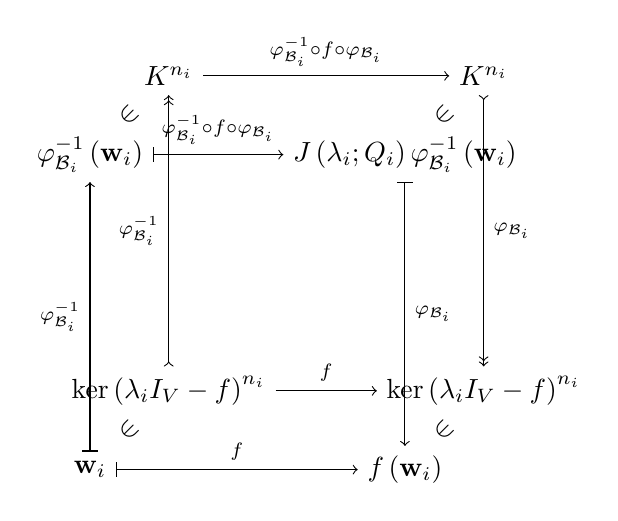
\begin{tikzpicture}[auto]

    \node (a) at (1, 1) {${\rm ker} \left( \lambda_i I_V -f\right) ^{n_i } $};
    \node (b) at (5, 1) {${\rm ker} \left( \lambda_i I_V -f\right) ^{n_i } $};
    \node (c) at (1, 5) {$K^{n_i } $};
    \node (d) at (5, 5) {$K^{n_i } $};
    \node (e) at (0, 4) {$\varphi_{{\mathcal B}_i }^{-1} \left( {\bf w}_i \right) $};
    \node (f) at (4, 4) {$J\left( \lambda_i ;Q_i \right) \varphi_{{\mathcal B}_i }^{-1} \left( {\bf w}_i \right) $};
    \node (g) at (0.5, 4.5) {\rotatebox{45}{$\scriptsize \in $} };
    \node (h) at (4.5, 4.5) {\rotatebox{45}{$\scriptsize \in $} };
    \node (i) at (0, 0) {${\bf w}_i $};
    \node (j) at (4, 0) {$f \left( {\bf w}_i \right) $};
    \node (k) at (0.5, 0.5) {\rotatebox{45}{$\in $} };
    \node (l) at (4.5, 0.5) {\rotatebox{45}{$\in $} };
    
    \draw [->] (c) to node {$\scriptstyle \varphi_{{\mathcal B}_i }^{-1} \circ f\circ \varphi_{{\mathcal B}_i } $} (d);
    \draw [|->] (e) to node {$\scriptstyle \varphi_{{\mathcal B}_i }^{-1} \circ f\circ \varphi_{{\mathcal B}_i } $} (f);
    \draw [>->>] (a) to node {$\scriptstyle \varphi_{{\mathcal B}_i }^{-1} $} (c);
    \draw [|->] (i) to node {$\scriptstyle \varphi_{{\mathcal B}_i }^{-1} $} (e);
    \draw [->] (a) to node {$\scriptstyle f$} (b);
    \draw [|->] (i) to node {$\scriptstyle f$} (j);
    \draw [>->>] (d) to node {$\scriptstyle \varphi_{{\mathcal B}_i } $} (b);
    \draw [|->] (f) to node {$\scriptstyle \varphi_{{\mathcal B}_i } $} (j);
    
  \end{tikzpicture} 
\end{center}
したがって、次のようになり、
\begin{center}
  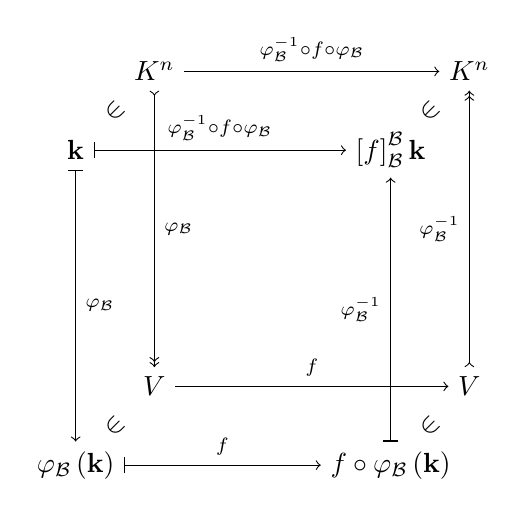
\begin{tikzpicture}[auto]

    \node (a) at (1, 1) {$V$};
    \node (b) at (5, 1) {$V$};
    \node (c) at (1, 5) {$K^n $};
    \node (d) at (5, 5) {$K^n $};
    \node (e) at (0, 4) {${\bf k} $};
    \node (f) at (4, 4) {$\left[ f\right]_{\mathcal B}^{\mathcal B} {\bf k} $};
    \node (g) at (0.5, 4.5) {\rotatebox{45}{$\scriptsize \in $} };
    \node (h) at (4.5, 4.5) {\rotatebox{45}{$\scriptsize \in $} };
    \node (i) at (0, 0) {$\varphi_{\mathcal B} \left( {\bf k} \right) $};
    \node (j) at (4, 0) {$f\circ \varphi_{\mathcal B} \left( {\bf k} \right) $};
    \node (k) at (0.5, 0.5) {\rotatebox{45}{$\in $} };
    \node (l) at (4.5, 0.5) {\rotatebox{45}{$\in $} };
    
    \draw [->] (c) to node {$\scriptstyle \varphi_{\mathcal B}^{-1} \circ f\circ \varphi_{\mathcal B} $} (d);
    \draw [|->] (e) to node {$\scriptstyle \varphi_{\mathcal B}^{-1} \circ f\circ \varphi_{\mathcal B} $} (f);
    \draw [>->>] (c) to node {$\scriptstyle \varphi_{\mathcal B} $} (a);
    \draw [|->] (e) to node {$\scriptstyle \varphi_{\mathcal B} $} (i);
    \draw [->] (a) to node {$\scriptstyle f$} (b);
    \draw [|->] (i) to node {$\scriptstyle f$} (j);
    \draw [>->>] (b) to node {$\scriptstyle \varphi_{\mathcal B}^{-1} $} (d);
    \draw [|->] (j) to node {$\scriptstyle \varphi_{\mathcal B}^{-1} $} (f);
    
  \end{tikzpicture} 
\end{center}  
したがって、次のようになる。
\begin{align*}
\varphi_{\mathcal{B}}^{- 1} \circ f \circ \varphi_{\mathcal{B}}\left( \mathbf{k} \right) &= \varphi_{\mathcal{B}}^{- 1} \circ f\left( \bigoplus_{i \in \varLambda_{s}} \mathbf{w}_{i} \right)\\
&= \sum_{i \in \varLambda_{s}} {\varphi_{\mathcal{B}}^{- 1} \circ f\left( \mathbf{w}_{i} \right)}\\
&= \sum_{i \in \varLambda_{s}} {\varphi_{\mathcal{B}}^{- 1} \circ \varphi_{\mathcal{B}_{i}}\left( J\left( \lambda_{i};Q_{i} \right)\varphi_{\mathcal{B}_{i}}^{- 1}\left( \mathbf{w}_{i} \right) \right)}\\
&= \varphi_{\mathcal{B}}^{- 1} \circ \varphi_{\mathcal{B}_{1}}\left( J\left( \lambda_{1};Q_{1} \right)\varphi_{\mathcal{B}_{1}}^{- 1}\left( \mathbf{w}_{1} \right) \right) + \varphi_{\mathcal{B}}^{- 1} \circ \varphi_{\mathcal{B}_{2}}\left( J\left( \lambda_{2};Q_{2} \right)\varphi_{\mathcal{B}_{2}}^{- 1}\left( \mathbf{w}_{2} \right) \right) + \cdots + \varphi_{\mathcal{B}}^{- 1} \circ \varphi_{\mathcal{B}_{s}}\left( J\left( \lambda_{s};Q_{s} \right)\varphi_{\mathcal{B}_{s}}^{- 1}\left( \mathbf{w}_{s} \right) \right)\\
&= \begin{pmatrix}
J\left( \lambda_{1};Q_{1} \right)\varphi_{\mathcal{B}_{1}}^{- 1}\left( \mathbf{w}_{1} \right) \\
\mathbf{0} \\
 \vdots \\
\mathbf{0} \\
\end{pmatrix} + \begin{pmatrix}
\mathbf{0} \\
J\left( \lambda_{2};Q_{2} \right)\varphi_{\mathcal{B}_{2}}^{- 1}\left( \mathbf{w}_{2} \right) \\
 \vdots \\
\mathbf{0} \\
\end{pmatrix} + \cdots + \begin{pmatrix}
\mathbf{0} \\
\mathbf{0} \\
 \vdots \\
J\left( \lambda_{s};Q_{s} \right)\varphi_{\mathcal{B}_{s}}^{- 1}\left( \mathbf{w}_{s} \right) \\
\end{pmatrix}\\
&= \begin{pmatrix}
J\left( \lambda_{1};Q_{1} \right) \\
O \\
 \vdots \\
O \\
\end{pmatrix}\varphi_{\mathcal{B}_{1}}^{- 1}\left( \mathbf{w}_{1} \right) + \begin{pmatrix}
O \\
J\left( \lambda_{2};Q_{2} \right) \\
 \vdots \\
O \\
\end{pmatrix}\varphi_{\mathcal{B}_{2}}^{- 1}\left( \mathbf{w}_{2} \right) + \cdots + \begin{pmatrix}
O \\
O \\
 \vdots \\
J\left( \lambda_{s};Q_{s} \right) \\
\end{pmatrix}\varphi_{\mathcal{B}_{s}}^{- 1}\left( \mathbf{w}_{s} \right)\\
&= \begin{pmatrix}
J\left( \lambda_{1};Q_{1} \right) & \  & \  & O \\
\  & J\left( \lambda_{2};Q_{2} \right) & \  & \  \\
\  & \  & \ddots & \  \\
O & \  & \  & J\left( \lambda_{s};Q_{s} \right) \\
\end{pmatrix}\begin{pmatrix}
\varphi_{\mathcal{B}_{1}}^{- 1}\left( \mathbf{w}_{1} \right) \\
\varphi_{\mathcal{B}_{2}}^{- 1}\left( \mathbf{w}_{2} \right) \\
 \vdots \\
\varphi_{\mathcal{B}_{s}}^{- 1}\left( \mathbf{w}_{s} \right) \\
\end{pmatrix}
\end{align*}
ここで、次のようになるので、
\begin{align*}
\begin{pmatrix}
\varphi_{\mathcal{B}_{1}}^{- 1}\left( \mathbf{w}_{1} \right) \\
\varphi_{\mathcal{B}_{2}}^{- 1}\left( \mathbf{w}_{2} \right) \\
 \vdots \\
\varphi_{\mathcal{B}_{s}}^{- 1}\left( \mathbf{w}_{s} \right) \\
\end{pmatrix} &= \begin{pmatrix}
\varphi_{\mathcal{B}_{1}}^{- 1}\left( \mathbf{w}_{1} \right) \\
\mathbf{0} \\
 \vdots \\
\mathbf{0} \\
\end{pmatrix} + \begin{pmatrix}
\mathbf{0} \\
\varphi_{\mathcal{B}_{2}}^{- 1}\left( \mathbf{w}_{2} \right) \\
 \vdots \\
\mathbf{0} \\
\end{pmatrix} + \cdots + \begin{pmatrix}
\mathbf{0} \\
\mathbf{0} \\
 \vdots \\
\varphi_{\mathcal{B}_{s}}^{- 1}\left( \mathbf{w}_{s} \right) \\
\end{pmatrix}\\
&= \varphi_{\mathcal{B}}^{- 1}\left( \mathbf{w}_{1} \right) + \varphi_{\mathcal{B}}^{- 1}\left( \mathbf{w}_{2} \right) + \cdots + \varphi_{\mathcal{B}}^{- 1}\left( \mathbf{w}_{s} \right)\\
&= \varphi_{\mathcal{B}}^{- 1}\left( \bigoplus_{j \in \varLambda_{s}} \mathbf{w}_{j} \right)\\
&= \varphi_{\mathcal{B}}^{- 1} \circ \varphi_{\mathcal{B}}\left( \mathbf{k} \right) = \mathbf{k}
\end{align*}
次のようになる。
\begin{align*}
\varphi_{\mathcal{B}}^{- 1} \circ f \circ \varphi_{\mathcal{B}}\left( \mathbf{k} \right) = \begin{pmatrix}
J\left( \lambda_{1};Q_{1} \right) & \  & \  & O \\
\  & J\left( \lambda_{2};Q_{2} \right) & \  & \  \\
\  & \  & \ddots & \  \\
O & \  & \  & J\left( \lambda_{s};Q_{s} \right) \\
\end{pmatrix}\mathbf{k}
\end{align*}
以上より、その表現行列$[ f]_{\mathcal{B}}^{\mathcal{B}}$が次式のように表されることができる。
\begin{align*}
[ f]_{\mathcal{B}}^{\mathcal{B}} = \begin{pmatrix}
J\left( \lambda_{1};Q_{1} \right) & \  & \  & O \\
\  & J\left( \lambda_{2};Q_{2} \right) & \  & \  \\
\  & \  & \ddots & \  \\
O & \  & \  & J\left( \lambda_{s};Q_{s} \right) \\
\end{pmatrix}
\end{align*}\par
ここで、行列たち$J\left( \lambda_{i};Q_{i} \right)$は定理\ref{2.2.6.1}より1つの固有値$\lambda_{i}$に対し一意的に決まるので、固有値$\lambda_{i}$の順序を除けば、即ち、その表現行列$[ f]_{\mathcal{B}}^{\mathcal{B}}$の中に入っているJordan塊たちの順序を除けば、その表現行列$[ f]_{\mathcal{B}}^{\mathcal{B}}$はその線形写像$f$に対し一意的に決まる。
\end{proof}
\begin{thm}\label{2.2.6.3}
代数的閉体$K$上の$n$次元vector空間$V$における線形写像$f:V \rightarrow V$の固有多項式$\varPhi_{f}$が互いに異なるその体$K$の元々$\lambda_{i}$を用いて$\sum_{i \in \varLambda_{s}} n_{i} = n$として次式のように表されることができるので、そうするとき、
\begin{align*}
\varPhi_{f} = \prod_{i \in \varLambda_{s}} \left( X - \lambda_{i} \right)^{n_{i}}
\end{align*}
次のことが成り立つ。
\begin{itemize}
\item
  $\forall i \in \varLambda_{s}$に対し、その線形写像$f$のJordan標準形に入っている固有値$\lambda_{i}$に対するJordan細胞$J\left( \lambda_{i},q_{ij} \right)$の個数$r_{i}$は冪零変換$\lambda_{i}I_{V} - f$の核の次元、即ち、その固有値$\lambda_{i}$に対する固有空間$W\left( \lambda_{i} \right)$の次元に等しい、即ち、次式が成り立つ。
\begin{align*}
r_{i} = {\mathrm{nullity}}\left( \lambda_{i}I_{V} - f \right) = \dim{W\left( \lambda_{i} \right)}
\end{align*}
\item
  $q_{i} = q_{i1}$として$\forall i \in \varLambda_{s}\forall j \in \varLambda_{q_{i}}$に対し、その線形写像$f$のJordan標準形に入っている固有値$\lambda_{i}$に対するJordan細胞$J\left( \lambda_{i},j \right)$の個数$\varepsilon_{ij}$は次式を満たす。
\begin{align*}
\varepsilon_{ij} &= 2{\mathrm{nullity}}\left( \lambda_{i}I_{V} - f \right)^{j} - {\mathrm{nullity}}\left( \lambda_{i}I_{V} - f \right)^{j + 1} - {\mathrm{nullity}}\left( \lambda_{i}I_{V} - f \right)^{j - 1}\\
&= {\mathrm{rank}}\left( \lambda_{i}I_{V} - f \right)^{j + 1} + {\mathrm{rank}}\left( \lambda_{i}I_{V} - f \right)^{j - 1} - 2{\mathrm{rank}}\left( \lambda_{i}I_{V} - f \right)^{j}
\end{align*}
\item
  $q_{i} = q_{i1}$として$\forall i \in \varLambda_{s}\forall j \in \varLambda_{q_{i}}$に対し、その線形写像$f$のJordan標準形に入っている固有値$\lambda_{i}$に対する$j \leq k$なるJordan細胞$J\left( \lambda_{i},k \right)$の個数$E_{ij}$は次式を満たす。
\begin{align*}
E_{ij} = {\mathrm{rank}}\left( \lambda_{i}I_{V} - f \right)^{j - 1} - {\mathrm{rank}}\left( \lambda_{i}I_{V} - f \right)^{j}
\end{align*}
\end{itemize}
\end{thm}
\begin{proof}
代数的閉体$K$上の$n$次元vector空間$V$における線形写像$f:V \rightarrow V$の固有多項式$\varPhi_{f}$が互いに異なるその体$K$の元々$\lambda_{i}$を用いて$\sum_{i \in \varLambda_{s}} n_{i} = n$として次式のように表されることができるので、そうするとき、
\begin{align*}
\varPhi_{f} = \prod_{i \in \varLambda_{s}} \left( X - \lambda_{i} \right)^{n_{i}}
\end{align*}
$\forall i \in \varLambda_{s}$に対し、定理\ref{2.2.6.1}よりその核$\ker\left( \lambda_{i}I_{V} - f \right)^{n_{i}}$における冪零変換$\lambda_{i}I_{V} - f$の不変系$Q_{i}$が$Q_{i} = \left( q_{ij} \right)_{j \in \varLambda_{r_{i}}}$と与えられたらば、定理\ref{2.2.6.2}よりそのvector空間$V$のある基底$\left\langle \mathcal{B}_{i} \right\rangle_{i \in \varLambda_{s}}$が存在して、これが$\mathcal{B}$とおかれると、これに関する線形写像$f$の表現行列$[ f]_{\mathcal{B}}^{\mathcal{B}}$が次式のように表されることができる。
\begin{align*}
[ f]_{\mathcal{B}}^{\mathcal{B}} = \begin{pmatrix}
J\left( \lambda_{1};Q_{1} \right) & \  & \  & O \\
\  & J\left( \lambda_{2};Q_{2} \right) & \  & \  \\
\  & \  & \ddots & \  \\
O & \  & \  & J\left( \lambda_{s};Q_{s} \right) \\
\end{pmatrix}
\end{align*}
このとき、その線形写像$f$のJordan標準形に入っている固有値$\lambda_{i}$に対するJordan細胞$J\left( \lambda_{i},q_{ij} \right)$の個数$r_{i}$は定理\ref{2.2.5.7}よりその核$\ker\left( \lambda_{i}I_{V} - f \right)$の次元に等しい、特に、固有空間の定義よりその固有値$\lambda_{i}$に対する固有空間$W\left( \lambda_{i} \right)$の次元に等しい、即ち、次式が成り立つ。
\begin{align*}
r_{i} = {\mathrm{nullity}}\left( \lambda_{i}I_{V} - f \right) = \dim{W\left( \lambda_{i} \right)}
\end{align*}\par
$q_{i} = q_{i1}$として$\forall i \in \varLambda_{s}\forall j \in \varLambda_{q_{i}}$に対し、その線形写像$f$のJordan標準形に入っている固有値$\lambda_{i}$に対するJordan細胞$J\left( \lambda_{i},j \right)$の個数$\varepsilon_{ij}$について、定理\ref{2.2.6.2}よりその個数$\varepsilon_{ij}$はその冪零変換$\lambda_{i}I_{V} - f$の不変系$Q_{i}$の値域$\left\{ q_{ij} \right\}_{j \in \varLambda_{r_{i}}}$のうち自然数$j$が含まれる個数に等しいので、定理\ref{2.2.5.5}より次式が成り立つ。
\begin{align*}
\varepsilon_{ij} = 2{\mathrm{nullity}}\left( \lambda_{i}I_{V} - f \right)^{j} - {\mathrm{nullity}}\left( \lambda_{i}I_{V} - f \right)^{j + 1} - {\mathrm{nullity}}\left( \lambda_{i}I_{V} - f \right)^{j - 1}
\end{align*}
ここで、それらの線形写像たち$\left( \lambda_{i}I_{V} - f \right)^{j}$に関する次元公式より次のようになることから、
\begin{align*}
\varepsilon_{ij} &= 2{\mathrm{nullity}}\left( \lambda_{i}I_{V} - f \right)^{j} - {\mathrm{nullity}}\left( \lambda_{i}I_{V} - f \right)^{j + 1} - {\mathrm{nullity}}\left( \lambda_{i}I_{V} - f \right)^{j - 1}\\
&= 2\left( {\mathrm{rank}}\left( \lambda_{i}I_{V} - f \right)^{j} + {\mathrm{nullity}}\left( \lambda_{i}I_{V} - f \right)^{j} - {\mathrm{rank}}\left( \lambda_{i}I_{V} - f \right)^{j} \right) \\
&\quad - \left( {\mathrm{rank}}\left( \lambda_{i}I_{V} - f \right)^{j + 1} + {\mathrm{nullity}}\left( \lambda_{i}I_{V} - f \right)^{j + 1} - {\mathrm{rank}}\left( \lambda_{i}I_{V} - f \right)^{j + 1} \right) \\
&\quad - \left( {\mathrm{rank}}\left( \lambda_{i}I_{V} - f \right)^{j - 1} + {\mathrm{nullity}}\left( \lambda_{i}I_{V} - f \right)^{j - 1} - {\mathrm{rank}}\left( \lambda_{i}I_{V} - f \right)^{j - 1} \right)\\
&= 2\left( n - {\mathrm{rank}}\left( \lambda_{i}I_{V} - f \right)^{j} \right) - \left( n - {\mathrm{rank}}\left( \lambda_{i}I_{V} - f \right)^{j + 1} \right) - \left( n - {\mathrm{rank}}\left( \lambda_{i}I_{V} - f \right)^{j - 1} \right)\\
&= 2n - 2{\mathrm{rank}}\left( \lambda_{i}I_{V} - f \right)^{j} - n + {\mathrm{rank}}\left( \lambda_{i}I_{V} - f \right)^{j + 1} - n + {\mathrm{rank}}\left( \lambda_{i}I_{V} - f \right)^{j - 1}\\
&= {\mathrm{rank}}\left( \lambda_{i}I_{V} - f \right)^{j + 1} + {\mathrm{rank}}\left( \lambda_{i}I_{V} - f \right)^{j - 1} - 2{\mathrm{rank}}\left( \lambda_{i}I_{V} - f \right)^{j}
\end{align*}
次式が得られる。
\begin{align*}
\varepsilon_{ij} &= 2{\mathrm{nullity}}\left( \lambda_{i}I_{V} - f \right)^{j} - {\mathrm{nullity}}\left( \lambda_{i}I_{V} - f \right)^{j + 1} - {\mathrm{nullity}}\left( \lambda_{i}I_{V} - f \right)^{j - 1}\\
&= {\mathrm{rank}}\left( \lambda_{i}I_{V} - f \right)^{j + 1} + {\mathrm{rank}}\left( \lambda_{i}I_{V} - f \right)^{j - 1} - 2{\mathrm{rank}}\left( \lambda_{i}I_{V} - f \right)^{j}
\end{align*}\par
$q_{i} = q_{i1}$として$\forall i \in \varLambda_{s}\forall j \in \varLambda_{q_{i}}$に対し、その線形写像$f$のJordan標準形に入っている固有値$\lambda_{i}$に対する$j \leq k$なるJordan細胞$J\left( \lambda_{i},k \right)$の個数$E_{ij}$について、上記の議論により、次のようになる。
\begin{align*}
E_{ij} &= \sum_{k \in \varLambda_{q_{i}} \setminus \varLambda_{j - 1}} \varepsilon_{ik}\\
&= \sum_{k \in \varLambda_{q_{i}} \setminus \varLambda_{j - 1}} \left( {\mathrm{rank}}\left( \lambda_{i}I_{V} - f \right)^{k + 1} + {\mathrm{rank}}\left( \lambda_{i}I_{V} - f \right)^{k - 1} - 2{\mathrm{rank}}\left( \lambda_{i}I_{V} - f \right)^{k} \right)\\
&= \sum_{k \in \varLambda_{q_{i}} \setminus \varLambda_{j - 1}} \left( \left( {\mathrm{rank}}\left( \lambda_{i}I_{V} - f \right)^{k + 1} - {\mathrm{rank}}\left( \lambda_{i}I_{V} - f \right)^{k} \right) \right. \\
&\quad \left. - \left( {\mathrm{rank}}\left( \lambda_{i}I_{V} - f \right)^{k} - {\mathrm{rank}}\left( \lambda_{i}I_{V} - f \right)^{k - 1} \right) \right)\\
&= \sum_{k \in \varLambda_{q_{i}} \setminus \varLambda_{j - 1}} \left( {\mathrm{rank}}\left( \lambda_{i}I_{V} - f \right)^{k + 1} - {\mathrm{rank}}\left( \lambda_{i}I_{V} - f \right)^{k} \right) \\
&\quad - \sum_{k \in \varLambda_{q_{i}} \setminus \varLambda_{j - 1}} \left( {\mathrm{rank}}\left( \lambda_{i}I_{V} - f \right)^{k} - {\mathrm{rank}}\left( \lambda_{i}I_{V} - f \right)^{k - 1} \right)\\
&= \left( {\mathrm{rank}}\left( \lambda_{i}I_{V} - f \right)^{q_{i} + 1} - {\mathrm{rank}}\left( \lambda_{i}I_{V} - f \right)^{q_{i}} \right) \\
&\quad + \sum_{k \in \varLambda_{q_{i} - 1} \setminus \varLambda_{j - 1}} \left( {\mathrm{rank}}\left( \lambda_{i}I_{V} - f \right)^{k + 1} - {\mathrm{rank}}\left( \lambda_{i}I_{V} - f \right)^{k} \right) \\
&\quad - \sum_{k \in \varLambda_{q_{i}} \setminus \varLambda_{j}} \left( {\mathrm{rank}}\left( \lambda_{i}I_{V} - f \right)^{k} - {\mathrm{rank}}\left( \lambda_{i}I_{V} - f \right)^{k - 1} \right) \\
&\quad - \left( {\mathrm{rank}}\left( \lambda_{i}I_{V} - f \right)^{j} - {\mathrm{rank}}\left( \lambda_{i}I_{V} - f \right)^{j - 1} \right)\\
&= {\mathrm{rank}}\left( \lambda_{i}I_{V} - f \right)^{j - 1} - {\mathrm{rank}}\left( \lambda_{i}I_{V} - f \right)^{j} \\
&\quad + {\mathrm{rank}}\left( \lambda_{i}I_{V} - f \right)^{q_{i} + 1} - {\mathrm{rank}}\left( \lambda_{i}I_{V} - f \right)^{q_{i}} \\
&\quad + \sum_{k \in \varLambda_{q_{i}} \setminus \varLambda_{j}} \left( {\mathrm{rank}}\left( \lambda_{i}I_{V} - f \right)^{k} - {\mathrm{rank}}\left( \lambda_{i}I_{V} - f \right)^{k - 1} \right) \\
&\quad - \sum_{k \in \varLambda_{q_{i}} \setminus \varLambda_{j}} \left( {\mathrm{rank}}\left( \lambda_{i}I_{V} - f \right)^{k} - {\mathrm{rank}}\left( \lambda_{i}I_{V} - f \right)^{k - 1} \right)\\
&= {\mathrm{rank}}\left( \lambda_{i}I_{V} - f \right)^{j - 1} - {\mathrm{rank}}\left( \lambda_{i}I_{V} - f \right)^{j} \\
&\quad + {\mathrm{rank}}\left( \lambda_{i}I_{V} - f \right)^{q_{i} + 1} - {\mathrm{rank}}\left( \lambda_{i}I_{V} - f \right)^{q_{i}}\\
&= {\mathrm{rank}}\left( \lambda_{i}I_{V} - f \right)^{j - 1} - {\mathrm{rank}}\left( \lambda_{i}I_{V} - f \right)^{j} + {\mathrm{rank}}0 - {\mathrm{rank}}0\\
&= {\mathrm{rank}}\left( \lambda_{i}I_{V} - f \right)^{j - 1} - {\mathrm{rank}}\left( \lambda_{i}I_{V} - f \right)^{j}
\end{align*}
\end{proof}
\begin{thm}\label{2.2.6.4}
代数的閉体$K$上の$n$次元vector空間$V$における線形写像たち$f:V \rightarrow V$、$g:V \rightarrow V$の固有多項式たち$\varPhi_{f}$、$\varPhi_{g}$が互いに異なるその体$K$の元々$\lambda_{i}$、互いに異なるその体$K$の元々$\mu_{i}$を用いて$\sum_{i \in \varLambda_{s}} m_{i} = \sum_{i \in \varLambda_{t}} n_{i} = n$として次式のように表されることができるので、そうするとき、
\begin{align*}
\varPhi_{f} = \prod_{i \in \varLambda_{s}} \left( X - \lambda_{i} \right)^{m_{i}},\ \ \varPhi_{g} = \prod_{i \in \varLambda_{t}} \left( X - \mu_{i} \right)^{n_{i}}
\end{align*}
任意の基底たち$\alpha$、$\beta$に関するそれらの線形写像たち$f$、$g$の表現行列たち$[ f]_{\alpha}^{\alpha}$、$[ g]_{\beta}^{\beta}$が互いに相似であるならそのときに限り、それらの線形写像たち$f$、$g$のJordan標準形がこれに入っているJordan blockの順序の違いを除けば一致する。
\end{thm}
\begin{proof}
代数的閉体$K$上の$n$次元vector空間$V$における線形写像たち$f:V \rightarrow V$、$g:V \rightarrow V$の固有多項式たち$\varPhi_{f}$、$\varPhi_{g}$が互いに異なるその体$K$の元々$\lambda_{i}$、互いに異なるその体$K$の元々$\mu_{i}$を用いて$\sum_{i \in \varLambda_{s}} m_{i} = \sum_{i \in \varLambda_{t}} n_{i} = n$として次式のように表されることができるので、そうするとき、
\begin{align*}
\varPhi_{f} = \prod_{i \in \varLambda_{s}} \left( X - \lambda_{i} \right)^{m_{i}},\ \ \varPhi_{g} = \prod_{i \in \varLambda_{t}} \left( X - \mu_{i} \right)^{n_{i}}
\end{align*}
任意の基底たち$\alpha$、$\beta$に関するそれらの線形写像たち$f$、$g$の表現行列たち$[ f]_{\alpha}^{\alpha}$、$[ g]_{\beta}^{\beta}$が相似であるならそのときに限り、ある正則行列$P$が存在して$P[ f]_{\alpha}^{\alpha} = [ g]_{\beta}^{\beta}P$が成り立つ。このとき、対応する$n$次正方行列が$A$であるようなそのvector空間$K^{n}$間の線形写像が$L_{A}:K^{n} \rightarrow K^{n}$、それらの基底たち$\alpha$、$\beta$に関する基底変換における線形同型写像たち$\varphi_{\alpha}$、$\varphi_{\beta}$を用いて次式が成り立ち、
\begin{center}
  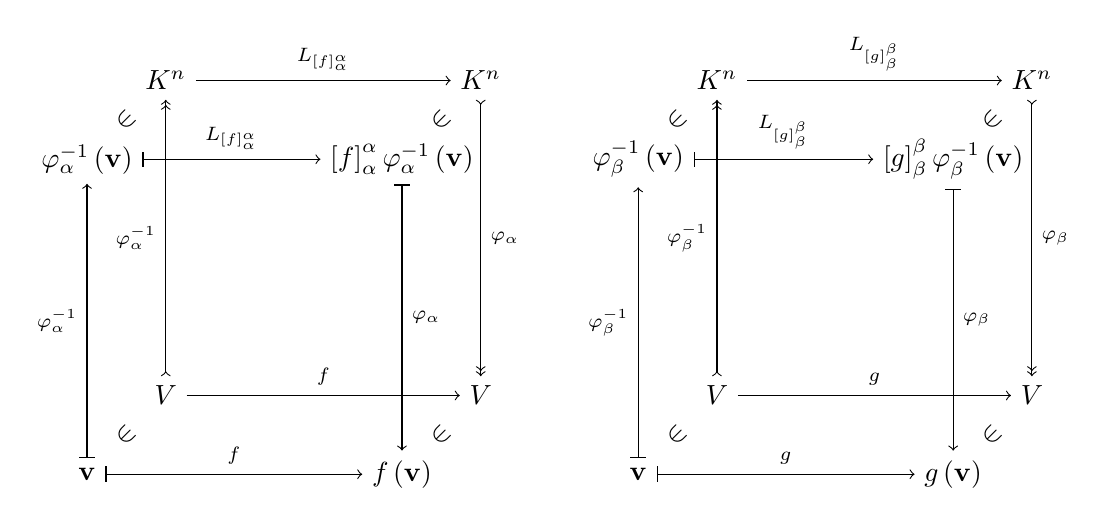
\begin{tikzpicture}[auto]

    \node (a) at (1, 1) {$V$};
    \node (b) at (5, 1) {$V$};
    \node (c) at (1, 5) {$K^n $};
    \node (d) at (5, 5) {$K^n $};
    \node (e) at (0, 4) {$\varphi_{\alpha }^{-1} \left( {\bf v} \right) $};
    \node (f) at (4, 4) {$\left[ f\right]_{\alpha }^{\alpha } \varphi_{\alpha }^{-1} \left( {\bf v} \right) $};
    \node (g) at (0.5, 4.5) {\rotatebox{45}{$\scriptsize \in $} };
    \node (h) at (4.5, 4.5) {\rotatebox{45}{$\scriptsize \in $} };
    \node (i) at (0, 0) {${\bf v} $};
    \node (j) at (4, 0) {$f \left( {\bf v} \right) $};
    \node (k) at (0.5, 0.5) {\rotatebox{45}{$\in $} };
    \node (l) at (4.5, 0.5) {\rotatebox{45}{$\in $} };
    
    \draw [->] (c) to node {$\scriptstyle L_{\left[ f\right]_{\alpha }^{\alpha } } $} (d);
    \draw [|->] (e) to node {$\scriptstyle L_{\left[ f\right]_{\alpha }^{\alpha } } $} (f);
    \draw [>->>] (a) to node {$\scriptstyle \varphi_{\alpha }^{-1} $} (c);
    \draw [|->] (i) to node {$\scriptstyle \varphi_{\alpha }^{-1} $} (e);
    \draw [->] (a) to node {$\scriptstyle f$} (b);
    \draw [|->] (i) to node {$\scriptstyle f$} (j);
    \draw [>->>] (d) to node {$\scriptstyle \varphi_{\alpha } $} (b);
    \draw [|->] (f) to node {$\scriptstyle \varphi_{\alpha } $} (j);

    \node (a) at (8, 1) {$V$};
    \node (b) at (12, 1) {$V$};
    \node (c) at (8, 5) {$K^n $};
    \node (d) at (12, 5) {$K^n $};
    \node (e) at (7, 4) {$\varphi_{\beta }^{-1} \left( {\bf v} \right) $};
    \node (f) at (11, 4) {$\left[ g\right]_{\beta }^{\beta } \varphi_{\beta }^{-1} \left( {\bf v} \right) $};
    \node (g) at (7.5, 4.5) {\rotatebox{45}{$\scriptsize \in $} };
    \node (h) at (11.5, 4.5) {\rotatebox{45}{$\scriptsize \in $} };
    \node (i) at (7, 0) {${\bf v} $};
    \node (j) at (11, 0) {$g \left( {\bf v} \right) $};
    \node (k) at (7.5, 0.5) {\rotatebox{45}{$\in $} };
    \node (l) at (11.5, 0.5) {\rotatebox{45}{$\in $} };
    
    \draw [->] (c) to node {$\scriptstyle L_{\left[ g\right]_{\beta }^{\beta } } $} (d);
    \draw [|->] (e) to node {$\scriptstyle L_{\left[ g\right]_{\beta }^{\beta } } $} (f);
    \draw [>->>] (a) to node {$\scriptstyle \varphi_{\beta }^{-1} $} (c);
    \draw [|->] (i) to node {$\scriptstyle \varphi_{\beta }^{-1} $} (e);
    \draw [->] (a) to node {$\scriptstyle g $} (b);
    \draw [|->] (i) to node {$\scriptstyle g $} (j);
    \draw [>->>] (d) to node {$\scriptstyle \varphi_{\beta } $} (b);
    \draw [|->] (f) to node {$\scriptstyle \varphi_{\beta } $} (j);
    
  \end{tikzpicture} 
\end{center}
これにより、$[ f]_{\alpha}^{\alpha} = P^{- 1}[ g]_{\beta}^{\beta}P$が成り立つことになり、線形同型写像$L_{P}$を用いて次式が成り立つ。
\begin{align*}
L_{[ f]_{\alpha}^{\alpha}} &= L_{P^{- 1}[ g]_{\beta}^{\beta}P}\\
&= L_{P^{- 1}} \circ L_{[ g]_{\beta}^{\beta}} \circ L_{P}\\
&= L_{P}^{- 1} \circ L_{[ g]_{\beta}^{\beta}} \circ L_{P}
\end{align*}
したがって、次式が成り立つ。
\begin{center}
  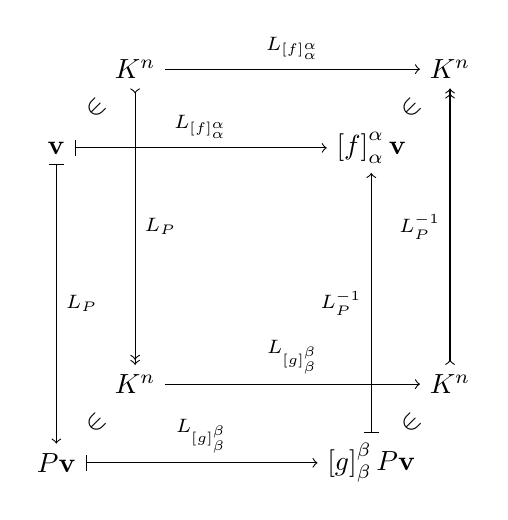
\begin{tikzpicture}[auto]

    \node (a) at (1, 1) {$K^n $};
    \node (b) at (5, 1) {$K^n $};
    \node (c) at (1, 5) {$K^n $};
    \node (d) at (5, 5) {$K^n $};
    \node (e) at (0, 4) {${\bf v} $};
    \node (f) at (4, 4) {$\left[ f\right]_{\alpha }^{\alpha } {\bf v} $};
    \node (g) at (0.5, 4.5) {\rotatebox{45}{$\scriptsize \in $} };
    \node (h) at (4.5, 4.5) {\rotatebox{45}{$\scriptsize \in $} };
    \node (i) at (0, 0) {$P{\bf v} $};
    \node (j) at (4, 0) {$\left[ g\right]_{\beta }^{\beta } P{\bf v} $};
    \node (k) at (0.5, 0.5) {\rotatebox{45}{$\in $} };
    \node (l) at (4.5, 0.5) {\rotatebox{45}{$\in $} };
    
    \draw [->] (c) to node {$\scriptstyle L_{\left[ f\right]_{\alpha }^{\alpha } } $} (d);
    \draw [|->] (e) to node {$\scriptstyle L_{\left[ f\right]_{\alpha }^{\alpha } } $} (f);
    \draw [>->>] (c) to node {$\scriptstyle L_P $} (a);
    \draw [|->] (e) to node {$\scriptstyle L_P $} (i);
    \draw [->] (a) to node {$\scriptstyle L_{\left[ g\right]_{\beta }^{\beta } } $} (b);
    \draw [|->] (i) to node {$\scriptstyle L_{\left[ g\right]_{\beta }^{\beta } } $} (j);
    \draw [>->>] (b) to node {$\scriptstyle L_P^{-1} $} (d);
    \draw [|->] (j) to node {$\scriptstyle L_P^{-1} $} (f);
    
  \end{tikzpicture} 
\end{center}
これにより、次式が成り立つ。
\begin{center}
  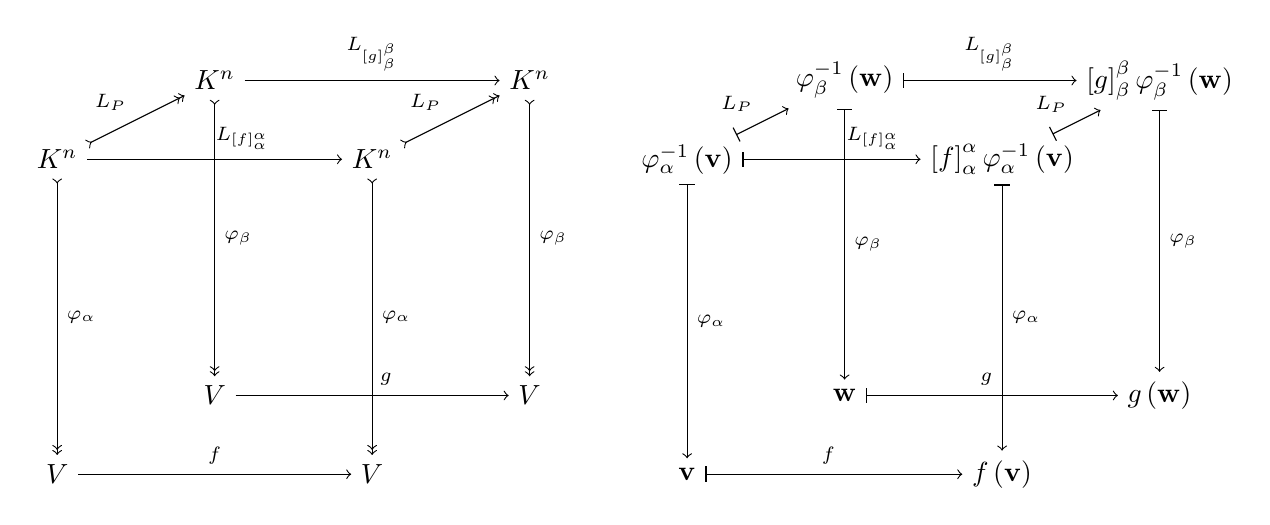
\begin{tikzpicture}[auto]

    \node (e) at (0, 0) {$V$};
    \node (f) at (4, 0) {$V$};
    \node (g) at (2, 1) {$V$};
    \node (h) at (6, 1) {$V$};
    \node (i) at (0, 4) {$K^n $};
    \node (j) at (4, 4) {$K^n $};
    \node (k) at (2, 5) {$K^n $};
    \node (l) at (6, 5) {$K^n $};
    
    \draw [->] (e) to node[xshift=0pt, yshift=0pt] {$\scriptstyle f$} (f);
    \draw [->] (g) to node[xshift=5pt, yshift=0pt] {$\scriptstyle g$} (h);
    \draw [->] (i) to node[xshift=10pt, yshift=0pt] {$\scriptstyle L_{\left[ f\right]_{\alpha }^{\alpha } } $} (j);
    \draw [->] (k) to node {$\scriptstyle L_{\left[ g\right]_{\beta }^{\beta } } $} (l);
    \draw [>->>] (i) to node {$\scriptstyle \varphi_{\alpha } $} (e);
    \draw [>->>] (j) to node {$\scriptstyle \varphi_{\alpha } $} (f);
    \draw [>->>] (k) to node {$\scriptstyle \varphi_{\beta } $} (g);
    \draw [>->>] (l) to node {$\scriptstyle \varphi_{\beta } $} (h);
    \draw [>->>] (i) to node {$\scriptstyle L_P $} (k);
    \draw [>->>] (j) to node {$\scriptstyle L_P $} (l);
    
    \node (e) at (8, 0) {${\bf v} $};
    \node (f) at (12, 0) {$f\left( {\bf v} \right) $};
    \node (g) at (10, 1) {${\bf w} $};
    \node (h) at (14, 1) {$g\left( {\bf w} \right) $};
    \node (i) at (8, 4) {$\varphi_{\alpha }^{-1} \left( {\bf v} \right) $};
    \node (j) at (12, 4) {$\left[ f\right]_{\alpha }^{\alpha } \varphi_{\alpha }^{-1} \left( {\bf v} \right) $};
    \node (k) at (10, 5) {$\varphi_{\beta }^{-1} \left( {\bf w} \right) $};
    \node (l) at (14, 5) {$\left[ g\right]_{\beta }^{\beta } \varphi_{\beta }^{-1} \left( {\bf w} \right) $};
    
    \draw [|->] (e) to node[xshift=-2pt, yshift=0pt] {$\scriptstyle f$} (f);
    \draw [|->] (g) to node[xshift=-2pt, yshift=0pt] {$\scriptstyle g$} (h);
    \draw [|->] (i) to node[xshift=15pt, yshift=0pt] {$\scriptstyle L_{\left[ f\right]_{\alpha }^{\alpha } } $} (j);
    \draw [|->] (k) to node {$\scriptstyle L_{\left[ g\right]_{\beta }^{\beta } } $} (l);
    \draw [|->] (i) to node {$\scriptstyle \varphi_{\alpha } $} (e);
    \draw [|->] (j) to node {$\scriptstyle \varphi_{\alpha } $} (f);
    \draw [|->] (k) to node {$\scriptstyle \varphi_{\beta } $} (g);
    \draw [|->] (l) to node {$\scriptstyle \varphi_{\beta } $} (h);
    \draw [|->] (i) to node {$\scriptstyle L_P $} (k);
    \draw [|->] (j) to node {$\scriptstyle L_P $} (l);
    
  \end{tikzpicture} 
\end{center}
$\forall i \in \varLambda_{s}$に対し、定理\ref{2.2.6.1}よりその核$\ker\left( \lambda_{i}I_{V} - f \right)^{n_{i}}$における冪零変換$\lambda_{i}I_{V} - f$の不変系$Q_{i}$が$Q_{i} = \left( q_{ij} \right)_{j \in \varLambda_{r_{i}}}$と与えられたらば、定理\ref{2.2.6.2}よりそのvector空間$V$のある基底$\left\langle \mathcal{B}_{i} \right\rangle_{i \in \varLambda_{s}}$が存在して、これが$\mathcal{B}$とおかれると、これに関する線形写像$f$の表現行列$[ f]_{\mathcal{B}}^{\mathcal{B}}$が次式のように表されることができる。
\begin{align*}
[ f]_{\mathcal{B}}^{\mathcal{B}} = \begin{pmatrix}
J\left( \lambda_{1};Q_{1} \right) & \  & \  & O \\
\  & J\left( \lambda_{2};Q_{2} \right) & \  & \  \\
\  & \  & \ddots & \  \\
O & \  & \  & J\left( \lambda_{s};Q_{s} \right) \\
\end{pmatrix}
\end{align*}
このとき、その基底$\mathcal{B}$に関する基底変換における線形同型写像$\varphi_{\mathcal{B}}$を用いて次式が成り立つ。
\begin{center}
  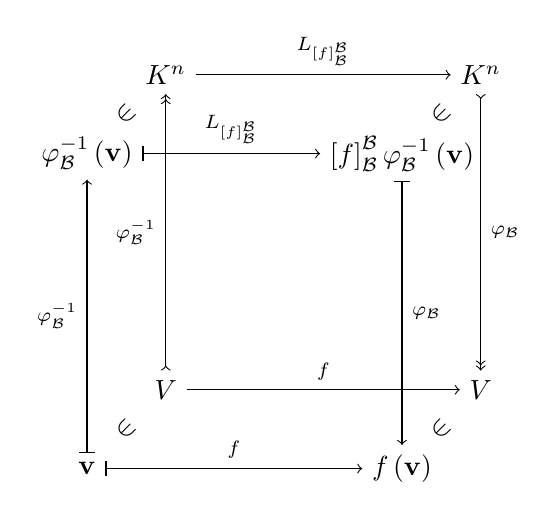
\begin{tikzpicture}[auto]

    \node (a) at (1, 1) {$V$};
    \node (b) at (5, 1) {$V$};
    \node (c) at (1, 5) {$K^n $};
    \node (d) at (5, 5) {$K^n $};
    \node (e) at (0, 4) {$\varphi_{{\mathcal B} }^{-1} \left( {\bf v} \right) $};
    \node (f) at (4, 4) {$\left[ f\right]_{{\mathcal B} }^{{\mathcal B} } \varphi_{{\mathcal B} }^{-1} \left( {\bf v} \right) $};
    \node (g) at (0.5, 4.5) {\rotatebox{45}{$\scriptsize \in $} };
    \node (h) at (4.5, 4.5) {\rotatebox{45}{$\scriptsize \in $} };
    \node (i) at (0, 0) {${\bf v} $};
    \node (j) at (4, 0) {$f \left( {\bf v} \right) $};
    \node (k) at (0.5, 0.5) {\rotatebox{45}{$\in $} };
    \node (l) at (4.5, 0.5) {\rotatebox{45}{$\in $} };
    
    \draw [->] (c) to node {$\scriptstyle L_{\left[ f\right]_{{\mathcal B} }^{{\mathcal B} } } $} (d);
    \draw [|->] (e) to node {$\scriptstyle L_{\left[ f\right]_{{\mathcal B} }^{{\mathcal B} } } $} (f);
    \draw [>->>] (a) to node {$\scriptstyle \varphi_{{\mathcal B} }^{-1} $} (c);
    \draw [|->] (i) to node {$\scriptstyle \varphi_{{\mathcal B} }^{-1} $} (e);
    \draw [->] (a) to node {$\scriptstyle f $} (b);
    \draw [|->] (i) to node {$\scriptstyle f $} (j);
    \draw [>->>] (d) to node {$\scriptstyle \varphi_{{\mathcal B} } $} (b);
    \draw [|->] (f) to node {$\scriptstyle \varphi_{{\mathcal B} } $} (j);
    
  \end{tikzpicture}
\end{center}
以上より、次式が成り立つ。
\begin{center}
  \begin{tikzpicture}[auto]

    \node (a) at (0, 0) {$K^n $};
    \node (b) at (4, 0) {$K^n $};
    \node (e) at (0, 4) {$V$};
    \node (f) at (4, 4) {$V$};
    \node (g) at (2, 5) {$V$};
    \node (h) at (6, 5) {$V$};
    \node (i) at (0, 8) {$K^n $};
    \node (j) at (4, 8) {$K^n $};
    \node (k) at (2, 9) {$K^n $};
    \node (l) at (6, 9) {$K^n $};
    
    \draw [->] (a) to node {$\scriptstyle L_{\left[ f\right]_{\mathcal B}^{\mathcal B} } $} (b);
    \draw [->] (e) to node[xshift=0pt, yshift=0pt] {$\scriptstyle f$} (f);
    \draw [->] (g) to node[xshift=5pt, yshift=0pt] {$\scriptstyle g$} (h);
    \draw [->] (i) to node[xshift=10pt, yshift=0pt] {$\scriptstyle L_{\left[ f\right]_{\alpha }^{\alpha } } $} (j);
    \draw [->] (k) to node {$\scriptstyle L_{\left[ g\right]_{\beta }^{\beta } } $} (l);
    \draw [>->>] (a) to node {$\scriptstyle \varphi_{\mathcal B} $} (e);
    \draw [>->>] (b) to node {$\scriptstyle \varphi_{\mathcal B} $} (f);
    \draw [>->>] (i) to node {$\scriptstyle \varphi_{\alpha } $} (e);
    \draw [>->>] (j) to node {$\scriptstyle \varphi_{\alpha } $} (f);
    \draw [>->>] (k) to node {$\scriptstyle \varphi_{\beta } $} (g);
    \draw [>->>] (l) to node {$\scriptstyle \varphi_{\beta } $} (h);
    \draw [>->>] (i) to node {$\scriptstyle L_P $} (k);
    \draw [>->>] (j) to node {$\scriptstyle L_P $} (l);
    
    \node (a) at (8, 0) {$\varphi_{{\mathcal B} }^{-1} \left( {\bf v} \right) $};
    \node (b) at (12, 0) {$\left[ f\right]_{\mathcal B}^{\mathcal B} \varphi_{{\mathcal B} }^{-1} \left( {\bf v} \right) $};
    \node (e) at (8, 4) {${\bf v} $};
    \node (f) at (12, 4) {$f\left( {\bf v} \right) $};
    \node (g) at (10, 5) {${\bf w} $};
    \node (h) at (14, 5) {$g\left( {\bf w} \right) $};
    \node (i) at (8, 8) {$\varphi_{\alpha }^{-1} \left( {\bf v} \right) $};
    \node (j) at (12, 8) {$\left[ f\right]_{\alpha }^{\alpha } \varphi_{\alpha }^{-1} \left( {\bf v} \right) $};
    \node (k) at (10, 9) {$\varphi_{\beta }^{-1} \left( {\bf w} \right) $};
    \node (l) at (14, 9) {$\left[ g\right]_{\beta }^{\beta } \varphi_{\beta }^{-1} \left( {\bf w} \right) $};
    
    \draw [|->] (a) to node {$\scriptstyle L_{\left[ f\right]_{\mathcal B}^{\mathcal B} } $} (b);
    \draw [|->] (e) to node[xshift=0pt, yshift=0pt] {$\scriptstyle f$} (f);
    \draw [|->] (g) to node[xshift=-2pt, yshift=0pt] {$\scriptstyle g$} (h);
    \draw [|->] (i) to node[xshift=15pt, yshift=0pt] {$\scriptstyle L_{\left[ f\right]_{\alpha }^{\alpha } } $} (j);
    \draw [|->] (k) to node {$\scriptstyle L_{\left[ g\right]_{\beta }^{\beta } } $} (l);
    \draw [|->] (a) to node {$\scriptstyle \varphi_{\mathcal B} $} (e);
    \draw [|->] (b) to node {$\scriptstyle \varphi_{\mathcal B} $} (f);
    \draw [|->] (i) to node {$\scriptstyle \varphi_{\alpha } $} (e);
    \draw [|->] (j) to node {$\scriptstyle \varphi_{\alpha } $} (f);
    \draw [|->] (k) to node {$\scriptstyle \varphi_{\beta } $} (g);
    \draw [|->] (l) to node {$\scriptstyle \varphi_{\beta } $} (h);
    \draw [|->] (i) to node {$\scriptstyle L_P $} (k);
    \draw [|->] (j) to node {$\scriptstyle L_P $} (l);
    
  \end{tikzpicture} 
\end{center}
ここで、合成写像$\varphi_{\beta} \circ L_{P} \circ \varphi_{\alpha}^{- 1} \circ \varphi_{\mathcal{B}}$は線形同型写像であるから、この写像によるそのvector空間$K^{n}$の直交標準基底の像々はそのvector空間$V$の基底をなし、これが$\mathcal{C}$とおかれると、その基底$\mathcal{C}$に関する基底変換における線形同型写像$\varphi_{\mathcal{C}}$を用いて次式が成り立つ。
\begin{center}
  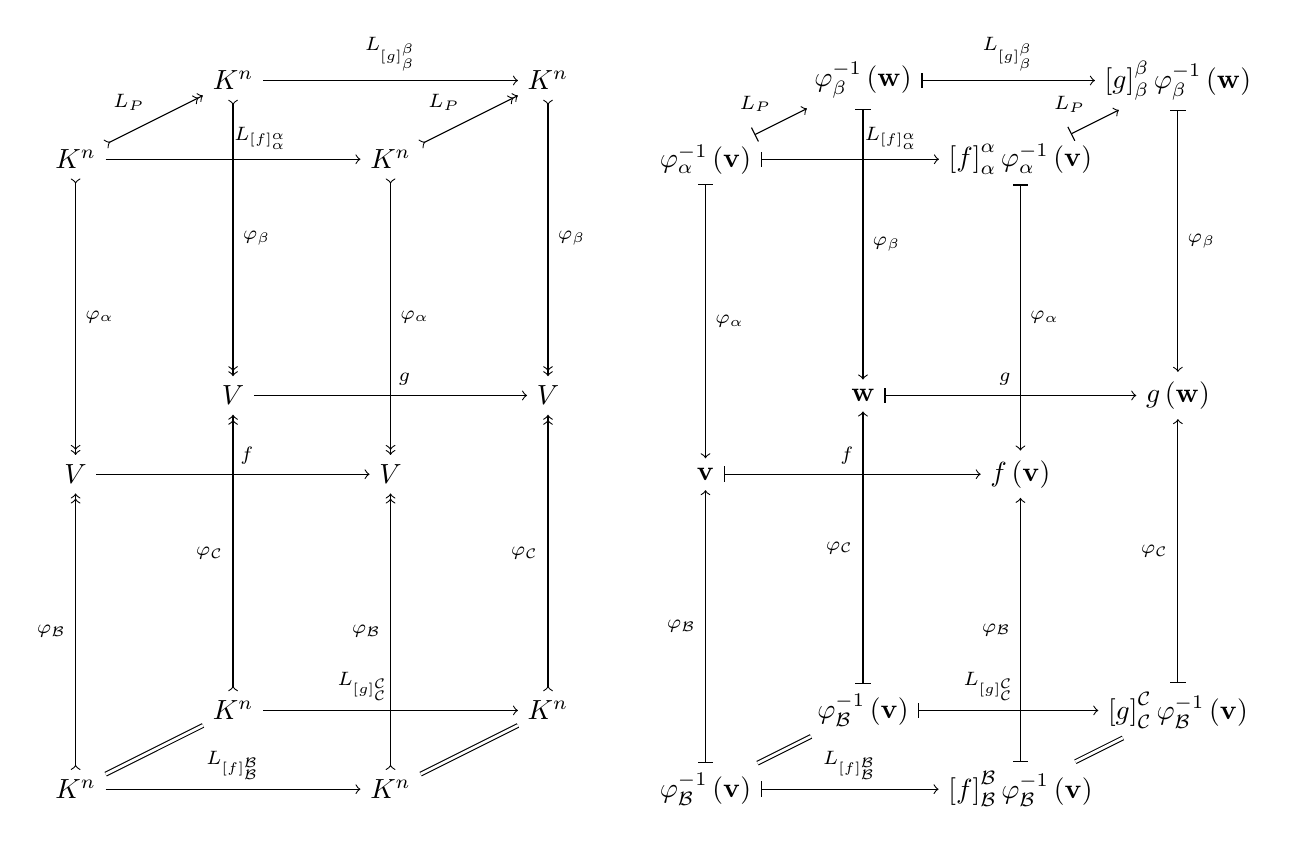
\begin{tikzpicture}[auto]

    \node (a) at (0, 0) {$K^n $};
    \node (b) at (4, 0) {$K^n $};
    \node (c) at (2, 1) {$K^n $};
    \node (d) at (6, 1) {$K^n $};
    \node (e) at (0, 4) {$V$};
    \node (f) at (4, 4) {$V$};
    \node (g) at (2, 5) {$V$};
    \node (h) at (6, 5) {$V$};
    \node (i) at (0, 8) {$K^n $};
    \node (j) at (4, 8) {$K^n $};
    \node (k) at (2, 9) {$K^n $};
    \node (l) at (6, 9) {$K^n $};
    
    \draw [->] (a) to node {$\scriptstyle L_{\left[ f\right]_{\mathcal B}^{\mathcal B} } $} (b);
    \draw [->] (c) to node[xshift=-10pt, yshift=0pt] {$\scriptstyle L_{\left[ g\right]_{\mathcal C}^{\mathcal C} } $} (d);
    \draw [->] (e) to node[xshift=5pt, yshift=0pt] {$\scriptstyle f$} (f);
    \draw [->] (g) to node[xshift=5pt, yshift=0pt] {$\scriptstyle g$} (h);
    \draw [->] (i) to node[xshift=10pt, yshift=0pt] {$\scriptstyle L_{\left[ f\right]_{\alpha }^{\alpha } } $} (j);
    \draw [->] (k) to node {$\scriptstyle L_{\left[ g\right]_{\beta }^{\beta } } $} (l);
    \draw [>->>] (a) to node {$\scriptstyle \varphi_{\mathcal B} $} (e);
    \draw [>->>] (b) to node {$\scriptstyle \varphi_{\mathcal B} $} (f);
    \draw [>->>] (c) to node {$\scriptstyle \varphi_{\mathcal C} $} (g);
    \draw [>->>] (d) to node {$\scriptstyle \varphi_{\mathcal C} $} (h);
    \draw [>->>] (i) to node {$\scriptstyle \varphi_{\alpha } $} (e);
    \draw [>->>] (j) to node {$\scriptstyle \varphi_{\alpha } $} (f);
    \draw [>->>] (k) to node {$\scriptstyle \varphi_{\beta } $} (g);
    \draw [>->>] (l) to node {$\scriptstyle \varphi_{\beta } $} (h);
    \draw [>->>] (i) to node {$\scriptstyle L_P $} (k);
    \draw [>->>] (j) to node {$\scriptstyle L_P $} (l);
    \draw [double distance=1pt] (a) to node {} (c);
    \draw [double distance=1pt] (b) to node {} (d);
    
    \node (a) at (8, 0) {$\varphi_{{\mathcal B} }^{-1} \left( {\bf v} \right) $};
    \node (b) at (12, 0) {$\left[ f\right]_{\mathcal B}^{\mathcal B} \varphi_{{\mathcal B} }^{-1} \left( {\bf v} \right) $};
    \node (c) at (10, 1) {$\varphi_{{\mathcal B} }^{-1} \left( {\bf v} \right) $};
    \node (d) at (14, 1) {$\left[ g\right]_{\mathcal C}^{\mathcal C} \varphi_{{\mathcal B} }^{-1} \left( {\bf v} \right) $};
    \node (e) at (8, 4) {${\bf v} $};
    \node (f) at (12, 4) {$f\left( {\bf v} \right) $};
    \node (g) at (10, 5) {${\bf w} $};
    \node (h) at (14, 5) {$g\left( {\bf w} \right) $};
    \node (i) at (8, 8) {$\varphi_{\alpha }^{-1} \left( {\bf v} \right) $};
    \node (j) at (12, 8) {$\left[ f\right]_{\alpha }^{\alpha } \varphi_{\alpha }^{-1} \left( {\bf v} \right) $};
    \node (k) at (10, 9) {$\varphi_{\beta }^{-1} \left( {\bf w} \right) $};
    \node (l) at (14, 9) {$\left[ g\right]_{\beta }^{\beta } \varphi_{\beta }^{-1} \left( {\bf w} \right) $};
    
    \draw [|->] (a) to node {$\scriptstyle L_{\left[ f\right]_{\mathcal B}^{\mathcal B} } $} (b);
    \draw [|->] (c) to node[xshift=-7pt, yshift=0pt] {$\scriptstyle L_{\left[ g\right]_{\mathcal C}^{\mathcal C} } $} (d);
    \draw [|->] (e) to node[xshift=-2pt, yshift=0pt] {$\scriptstyle f$} (f);
    \draw [|->] (g) to node[xshift=-2pt, yshift=0pt] {$\scriptstyle g$} (h);
    \draw [|->] (i) to node[xshift=15pt, yshift=0pt] {$\scriptstyle L_{\left[ f\right]_{\alpha }^{\alpha } } $} (j);
    \draw [|->] (k) to node {$\scriptstyle L_{\left[ g\right]_{\beta }^{\beta } } $} (l);
    \draw [|->] (a) to node {$\scriptstyle \varphi_{\mathcal B} $} (e);
    \draw [|->] (b) to node {$\scriptstyle \varphi_{\mathcal B} $} (f);
    \draw [|->] (c) to node {$\scriptstyle \varphi_{\mathcal C} $} (g);
    \draw [|->] (d) to node {$\scriptstyle \varphi_{\mathcal C} $} (h);
    \draw [|->] (i) to node {$\scriptstyle \varphi_{\alpha } $} (e);
    \draw [|->] (j) to node {$\scriptstyle \varphi_{\alpha } $} (f);
    \draw [|->] (k) to node {$\scriptstyle \varphi_{\beta } $} (g);
    \draw [|->] (l) to node {$\scriptstyle \varphi_{\beta } $} (h);
    \draw [|->] (i) to node {$\scriptstyle L_P $} (k);
    \draw [|->] (j) to node {$\scriptstyle L_P $} (l);
    \draw [double distance=1pt] (a) to node {} (c);
    \draw [double distance=1pt] (b) to node {} (d);
    
  \end{tikzpicture} 
\end{center}
これにより、その基底$\mathcal{C}$に関するその線形写像$g$の表現行列$[ g]_{\mathcal{C}}^{\mathcal{C}}$について、$[ f]_{\mathcal{B}}^{\mathcal{B}} = [ g]_{\mathcal{C}}^{\mathcal{C}}$が成り立つ。これにより、それらの線形写像たち$f$、$g$のJordan標準形がこれに入っているJordan blockの順序の違いを除けば一致する。\par
逆に、それらの線形写像たち$f$、$g$のJordan標準形がこれに入っているJordan blockの順序の違いを除けば一致するなら、任意の基底たち$\alpha$、$\beta$に関するそれらの線形写像たち$f$、$g$の表現行列たち$[ f]_{\alpha}^{\alpha}$、$[ g]_{\beta}^{\beta}$を用いて次式が成り立つ。
\begin{center}
  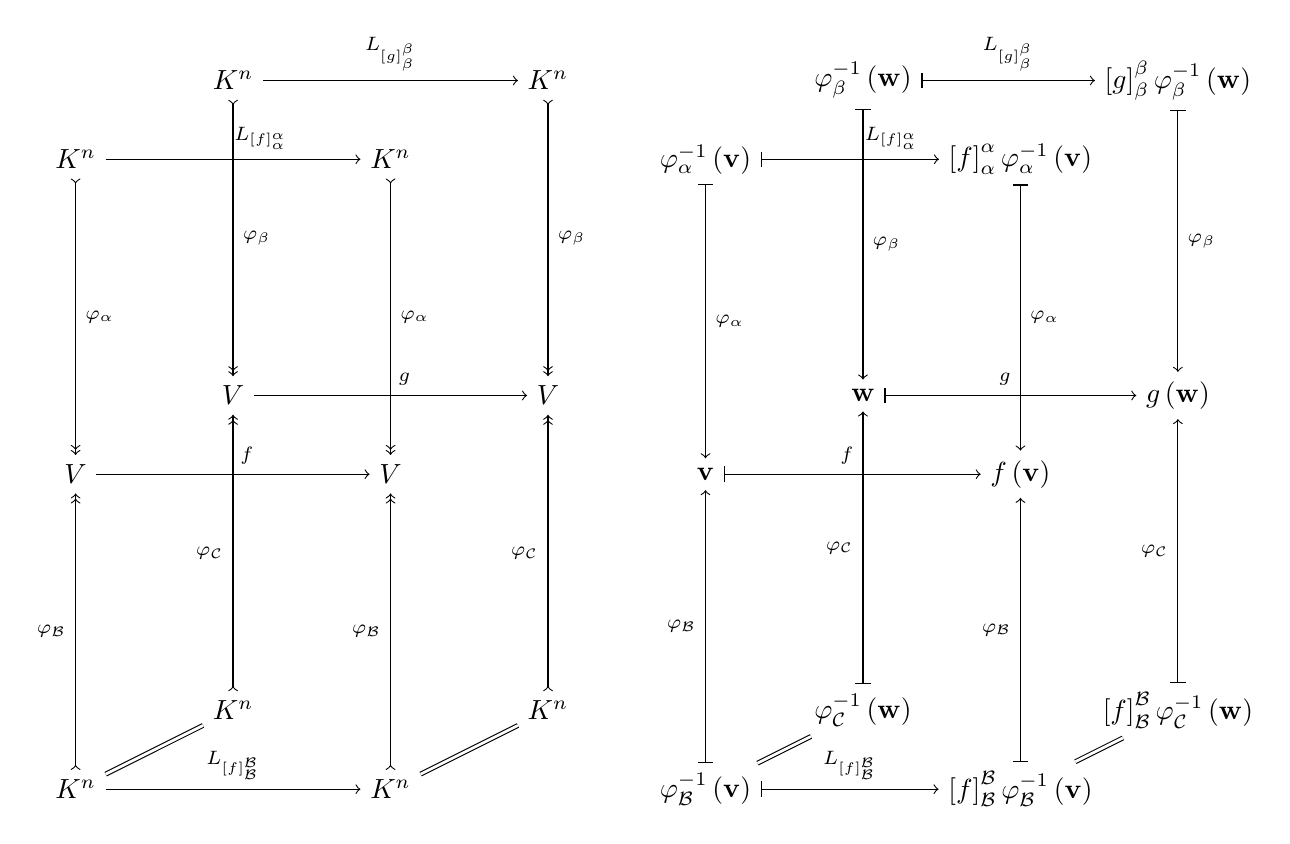
\begin{tikzpicture}[auto]

    \node (a) at (0, 0) {$K^n $};
    \node (b) at (4, 0) {$K^n $};
    \node (c) at (2, 1) {$K^n $};
    \node (d) at (6, 1) {$K^n $};
    \node (e) at (0, 4) {$V$};
    \node (f) at (4, 4) {$V$};
    \node (g) at (2, 5) {$V$};
    \node (h) at (6, 5) {$V$};
    \node (i) at (0, 8) {$K^n $};
    \node (j) at (4, 8) {$K^n $};
    \node (k) at (2, 9) {$K^n $};
    \node (l) at (6, 9) {$K^n $};
    
    \draw [->] (a) to node {$\scriptstyle L_{\left[ f\right]_{\mathcal B}^{\mathcal B} } $} (b);
    \draw [->] (e) to node[xshift=5pt, yshift=0pt] {$\scriptstyle f$} (f);
    \draw [->] (g) to node[xshift=5pt, yshift=0pt] {$\scriptstyle g$} (h);
    \draw [->] (i) to node[xshift=10pt, yshift=0pt] {$\scriptstyle L_{\left[ f\right]_{\alpha }^{\alpha } } $} (j);
    \draw [->] (k) to node {$\scriptstyle L_{\left[ g\right]_{\beta }^{\beta } } $} (l);
    \draw [>->>] (a) to node {$\scriptstyle \varphi_{\mathcal B} $} (e);
    \draw [>->>] (b) to node {$\scriptstyle \varphi_{\mathcal B} $} (f);
    \draw [>->>] (c) to node {$\scriptstyle \varphi_{\mathcal C} $} (g);
    \draw [>->>] (d) to node {$\scriptstyle \varphi_{\mathcal C} $} (h);
    \draw [>->>] (i) to node {$\scriptstyle \varphi_{\alpha } $} (e);
    \draw [>->>] (j) to node {$\scriptstyle \varphi_{\alpha } $} (f);
    \draw [>->>] (k) to node {$\scriptstyle \varphi_{\beta } $} (g);
    \draw [>->>] (l) to node {$\scriptstyle \varphi_{\beta } $} (h);
    \draw [double distance=1pt] (a) to node {} (c);
    \draw [double distance=1pt] (b) to node {} (d);
    
    \node (a) at (8, 0) {$\varphi_{{\mathcal B} }^{-1} \left( {\bf v} \right) $};
    \node (b) at (12, 0) {$\left[ f\right]_{\mathcal B}^{\mathcal B} \varphi_{{\mathcal B} }^{-1} \left( {\bf v} \right) $};
    \node (c) at (10, 1) {$\varphi_{{\mathcal C} }^{-1} \left( {\bf w} \right) $};
    \node (d) at (14, 1) {$\left[ f\right]_{\mathcal B}^{\mathcal B} \varphi_{{\mathcal C} }^{-1} \left( {\bf w} \right) $};
    \node (e) at (8, 4) {${\bf v} $};
    \node (f) at (12, 4) {$f\left( {\bf v} \right) $};
    \node (g) at (10, 5) {${\bf w} $};
    \node (h) at (14, 5) {$g\left( {\bf w} \right) $};
    \node (i) at (8, 8) {$\varphi_{\alpha }^{-1} \left( {\bf v} \right) $};
    \node (j) at (12, 8) {$\left[ f\right]_{\alpha }^{\alpha } \varphi_{\alpha }^{-1} \left( {\bf v} \right) $};
    \node (k) at (10, 9) {$\varphi_{\beta }^{-1} \left( {\bf w} \right) $};
    \node (l) at (14, 9) {$\left[ g\right]_{\beta }^{\beta } \varphi_{\beta }^{-1} \left( {\bf w} \right) $};
    
    \draw [|->] (a) to node {$\scriptstyle L_{\left[ f\right]_{\mathcal B}^{\mathcal B} } $} (b);
    \draw [|->] (e) to node[xshift=-2pt, yshift=0pt] {$\scriptstyle f$} (f);
    \draw [|->] (g) to node[xshift=-2pt, yshift=0pt] {$\scriptstyle g$} (h);
    \draw [|->] (i) to node[xshift=15pt, yshift=0pt] {$\scriptstyle L_{\left[ f\right]_{\alpha }^{\alpha } } $} (j);
    \draw [|->] (k) to node {$\scriptstyle L_{\left[ g\right]_{\beta }^{\beta } } $} (l);
    \draw [|->] (a) to node {$\scriptstyle \varphi_{\mathcal B} $} (e);
    \draw [|->] (b) to node {$\scriptstyle \varphi_{\mathcal B} $} (f);
    \draw [|->] (c) to node {$\scriptstyle \varphi_{\mathcal C} $} (g);
    \draw [|->] (d) to node {$\scriptstyle \varphi_{\mathcal C} $} (h);
    \draw [|->] (i) to node {$\scriptstyle \varphi_{\alpha } $} (e);
    \draw [|->] (j) to node {$\scriptstyle \varphi_{\alpha } $} (f);
    \draw [|->] (k) to node {$\scriptstyle \varphi_{\beta } $} (g);
    \draw [|->] (l) to node {$\scriptstyle \varphi_{\beta } $} (h);
    \draw [double distance=1pt] (a) to node {} (c);
    \draw [double distance=1pt] (b) to node {} (d);
    
    \end{tikzpicture} 
\end{center}
ここで、合成写像$\varphi_{\beta}^{- 1} \circ \varphi_{\mathcal{C}} \circ \varphi_{\mathcal{B}}^{- 1} \circ \varphi_{\alpha}$は線形同型写像であるから、これに対応する行列が$P$とおかれると、この行列$P$は正則行列で次式が成り立つ。
\begin{center}
  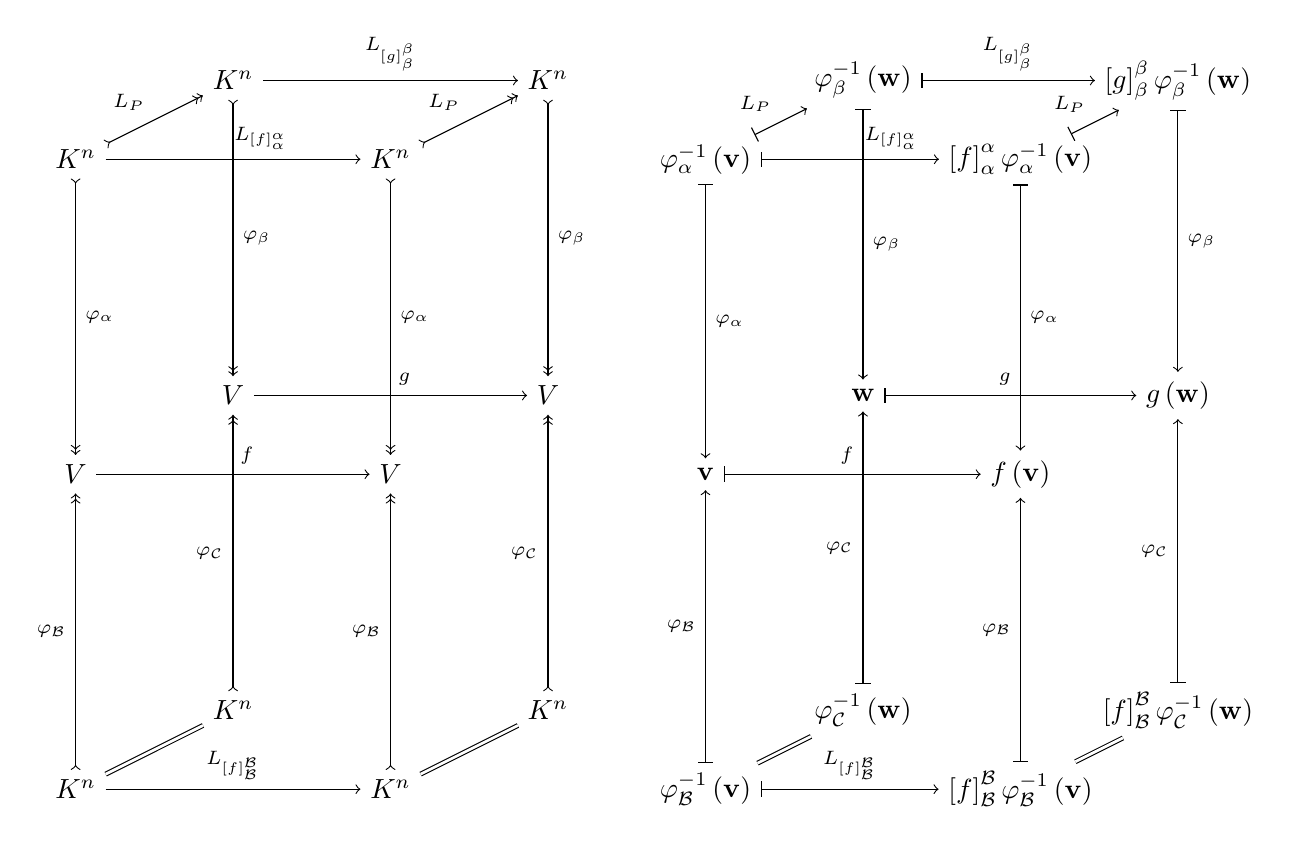
\begin{tikzpicture}[auto]

    \node (a) at (0, 0) {$K^n $};
    \node (b) at (4, 0) {$K^n $};
    \node (c) at (2, 1) {$K^n $};
    \node (d) at (6, 1) {$K^n $};
    \node (e) at (0, 4) {$V$};
    \node (f) at (4, 4) {$V$};
    \node (g) at (2, 5) {$V$};
    \node (h) at (6, 5) {$V$};
    \node (i) at (0, 8) {$K^n $};
    \node (j) at (4, 8) {$K^n $};
    \node (k) at (2, 9) {$K^n $};
    \node (l) at (6, 9) {$K^n $};
    
    \draw [->] (a) to node {$\scriptstyle L_{\left[ f\right]_{\mathcal B}^{\mathcal B} } $} (b);
    \draw [->] (e) to node[xshift=5pt, yshift=0pt] {$\scriptstyle f$} (f);
    \draw [->] (g) to node[xshift=5pt, yshift=0pt] {$\scriptstyle g$} (h);
    \draw [->] (i) to node[xshift=10pt, yshift=0pt] {$\scriptstyle L_{\left[ f\right]_{\alpha }^{\alpha } } $} (j);
    \draw [->] (k) to node {$\scriptstyle L_{\left[ g\right]_{\beta }^{\beta } } $} (l);
    \draw [>->>] (a) to node {$\scriptstyle \varphi_{\mathcal B} $} (e);
    \draw [>->>] (b) to node {$\scriptstyle \varphi_{\mathcal B} $} (f);
    \draw [>->>] (c) to node {$\scriptstyle \varphi_{\mathcal C} $} (g);
    \draw [>->>] (d) to node {$\scriptstyle \varphi_{\mathcal C} $} (h);
    \draw [>->>] (i) to node {$\scriptstyle \varphi_{\alpha } $} (e);
    \draw [>->>] (j) to node {$\scriptstyle \varphi_{\alpha } $} (f);
    \draw [>->>] (k) to node {$\scriptstyle \varphi_{\beta } $} (g);
    \draw [>->>] (l) to node {$\scriptstyle \varphi_{\beta } $} (h);
    \draw [>->>] (i) to node {$\scriptstyle L_P $} (k);
    \draw [>->>] (j) to node {$\scriptstyle L_P $} (l);
    \draw [double distance=1pt] (a) to node {} (c);
    \draw [double distance=1pt] (b) to node {} (d);
    
    \node (a) at (8, 0) {$\varphi_{{\mathcal B} }^{-1} \left( {\bf v} \right) $};
    \node (b) at (12, 0) {$\left[ f\right]_{\mathcal B}^{\mathcal B} \varphi_{{\mathcal B} }^{-1} \left( {\bf v} \right) $};
    \node (c) at (10, 1) {$\varphi_{{\mathcal C} }^{-1} \left( {\bf w} \right) $};
    \node (d) at (14, 1) {$\left[ f\right]_{\mathcal B}^{\mathcal B} \varphi_{{\mathcal C} }^{-1} \left( {\bf w} \right) $};
    \node (e) at (8, 4) {${\bf v} $};
    \node (f) at (12, 4) {$f\left( {\bf v} \right) $};
    \node (g) at (10, 5) {${\bf w} $};
    \node (h) at (14, 5) {$g\left( {\bf w} \right) $};
    \node (i) at (8, 8) {$\varphi_{\alpha }^{-1} \left( {\bf v} \right) $};
    \node (j) at (12, 8) {$\left[ f\right]_{\alpha }^{\alpha } \varphi_{\alpha }^{-1} \left( {\bf v} \right) $};
    \node (k) at (10, 9) {$\varphi_{\beta }^{-1} \left( {\bf w} \right) $};
    \node (l) at (14, 9) {$\left[ g\right]_{\beta }^{\beta } \varphi_{\beta }^{-1} \left( {\bf w} \right) $};
    
    \draw [|->] (a) to node {$\scriptstyle L_{\left[ f\right]_{\mathcal B}^{\mathcal B} } $} (b);
    \draw [|->] (e) to node[xshift=-2pt, yshift=0pt] {$\scriptstyle f$} (f);
    \draw [|->] (g) to node[xshift=-2pt, yshift=0pt] {$\scriptstyle g$} (h);
    \draw [|->] (i) to node[xshift=15pt, yshift=0pt] {$\scriptstyle L_{\left[ f\right]_{\alpha }^{\alpha } } $} (j);
    \draw [|->] (k) to node {$\scriptstyle L_{\left[ g\right]_{\beta }^{\beta } } $} (l);
    \draw [|->] (a) to node {$\scriptstyle \varphi_{\mathcal B} $} (e);
    \draw [|->] (b) to node {$\scriptstyle \varphi_{\mathcal B} $} (f);
    \draw [|->] (c) to node {$\scriptstyle \varphi_{\mathcal C} $} (g);
    \draw [|->] (d) to node {$\scriptstyle \varphi_{\mathcal C} $} (h);
    \draw [|->] (i) to node {$\scriptstyle \varphi_{\alpha } $} (e);
    \draw [|->] (j) to node {$\scriptstyle \varphi_{\alpha } $} (f);
    \draw [|->] (k) to node {$\scriptstyle \varphi_{\beta } $} (g);
    \draw [|->] (l) to node {$\scriptstyle \varphi_{\beta } $} (h);
    \draw [|->] (i) to node {$\scriptstyle L_P $} (k);
    \draw [|->] (j) to node {$\scriptstyle L_P $} (l);
    \draw [double distance=1pt] (a) to node {} (c);
    \draw [double distance=1pt] (b) to node {} (d);
    
  \end{tikzpicture} 
\end{center}
したがって、次式が成り立つ。
\begin{align*}
L_{[ f]_{\alpha}^{\alpha}} &= L_{P}^{- 1} \circ L_{[ g]_{\beta}^{\beta}} \circ L_{P}\\
&= L_{P^{- 1}} \circ L_{[ g]_{\beta}^{\beta}} \circ L_{P}\\
&= L_{P^{- 1}[ g]_{\beta}^{\beta}P}
\end{align*}
これにより、$[ f]_{\alpha}^{\alpha} = P^{- 1}[ g]_{\beta}^{\beta}P$が成り立つことになり、したがって、$P[ f]_{\alpha}^{\alpha} = [ g]_{\beta}^{\beta}P$が成り立つので、任意の基底たち$\alpha$、$\beta$に関するそれらの線形写像たち$f$、$g$の表現行列たち$[ f]_{\alpha}^{\alpha}$、$[ g]_{\beta}^{\beta}$は相似である。
\end{proof}
%\hypertarget{ux6700ux5c0fux591aux9805ux5f0f}{%
\subsubsection{最小多項式}%\label{ux6700ux5c0fux591aux9805ux5f0f}}
\begin{dfn}
Hamilton-Cayleyの定理より体$K$上の多項式環$K[ X]$の多項式$\rho$のうち、これに体$K$上の$n$次元vector空間$V$における線形写像$f:V \rightarrow V$を代入した写像$\rho(f)$が$\rho(f) = 0$を満たすものが存在するのであった。このようにその線形写像$f:V \rightarrow V$に対し、これを代入した写像が$0:V \rightarrow V$となるような多項式たちのうちもとの定数でない多項式の次数が最小で最高次の係数が$1$であるようなものをその線形写像$f$の最小多項式、これから定められる多項式写像をその線形写像$f$の最小多項式写像といい、ここでは、どちらも$\varphi_{f}$と書くことにする。
\end{dfn}
\begin{thm}\label{2.2.6.5}
体$K$上の多項式環$K[ X]$の元$\rho$の変数$X$にその体$K$上の$n$次元vector空間$V$における線形写像$f:V \rightarrow V$を代入した写像$\rho(f)$が$\rho(f) = 0$となるならそのときに限り、その線形写像$f$の最小多項式$\varphi_{f}$でその多項式$\rho$が割り切れる。
\end{thm}
\begin{proof}
体$K$上の多項式環$K[ X]$の元$\rho$の変数$X$にその体$K$上の$n$次元vector空間$V$における線形写像$f:V \rightarrow V$を代入した写像$\rho(f)$が$\rho(f) = 0$となるとき、その線形写像$f$の最小多項式$\varphi_{f}$でその多項式$\rho$が割られると、除法の定理より$\exists q,r \in K[ X]$に対し、$\rho = q\varphi_{f} + r$かつ$\deg{r} < \deg{\varphi_{f}}$が成り立つ。このとき、それらの多項式たち$q$、$r$から定義される多項式写像たち$q$、$r$を用いて$\rho = q\varphi_{f} + r$が成り立つ。したがって、次のようになる。
\begin{align*}
0 = \rho(f) = q(f) \circ \varphi_{f}(f) + r(f) = r(f)
\end{align*}
ここで、$0 < \deg{r}$とすれば、$\deg{r} < \deg{\varphi_{f}}$が成り立つかつ、$r(f) = 0$が成り立つので、その多項式$\varphi_{f}$がその線形写像$f$の最小多項式でないことになるが、これは仮定に矛盾する。さらに、$r \neq \overline{0}$とすれば、$r(f) \neq 0$が成り立ち、$r(f) = 0$が成り立つことに矛盾するので、$r = \overline{0}$が成り立つ。このとき、$\rho = q\varphi_{f}$が成り立つことになるので、その多項式$\varphi_{f}$でその多項式$\rho$が割り切れる。\par
逆に、その線形写像$f$の最小多項式$\varphi_{f}$でその多項式$\rho$が割り切れるなら、$\exists q \in K[ X]$に対し、$\rho = q\varphi_{f}$が成り立つので、$\rho = q\varphi_{f}$が成り立つ。ここで、$\varphi_{f}(f) = 0$が成り立つので、次のようになる。
\begin{align*}
\rho(f) = q(f) \circ \varphi_{f}(f) = 0
\end{align*}
\end{proof}
\begin{thm}\label{2.2.6.6}
体$K$上の$n$次元vector空間$V$における線形写像$f:V \rightarrow V$の最小多項式は一意的に存在する。
\end{thm}
\begin{proof}
体$K$上の$n$次元vector空間$V$における線形写像$f:V \rightarrow V$の最小多項式が$\varphi_{f}$、$\chi_{f}$と与えられたとする。定理\ref{2.2.6.5}より$\exists q,r \in K[ X]$に対し、$\varphi_{f} = q\chi_{f}$かつ$\chi_{f} = r\varphi_{f}$が成り立つ。このとき、$\deg{\varphi_{f}} = \deg{\chi_{f}}$が成り立つことにより、$\deg{q} = \deg{r} = 0$が成り立つので、$\exists a,b \in K$に対し、$q = \overline{a}$かつ$r = \overline{b}$が成り立つことになる。ここで、$a \neq 1$とすれば、次のようになることから、
\begin{align*}
\varphi_{f} &= q\chi_{f}\\
&= \overline{a}\sum_{i \in \varLambda_{\deg{\chi_{f}}} \cup \left\{ 0 \right\}} {\chi_{f}(i)X^{i}}\\
&= \sum_{i \in \varLambda_{\deg{\chi_{f}}} \cup \left\{ 0 \right\}} {\overline{a}\overline{\chi_{f}(i)}X^{i}}\\
&= \sum_{i \in \varLambda_{\deg{\chi_{f}}} \cup \left\{ 0 \right\}} {\overline{a\chi_{f}(i)}X^{i}}\\
&= \sum_{i \in \varLambda_{\deg{q\chi_{f}}} \cup \left\{ 0 \right\}} {\overline{\left( q\chi_{f} \right)(i)}X^{i}}
\end{align*}
その多項式$q\chi_{f}$の最高次の係数$\overline{\left( q\chi_{f} \right)\left( \deg{q\chi_{f}} \right)}$が$\overline{a\chi_{f}\left( \deg{\chi_{f}} \right)}$に等しいので、その最高次の係数は$\overline{1}$でないことになるが、$\varphi_{f} = q\chi_{f}$が成り立つことにより最小多項式写像の定義に矛盾する。したがって、$a = 1$が成り立つ。同様にして、$b = 1$が成り立つ。このとき、$\varphi_{f} = \chi_{f}$が成り立つので、その線形写像$f:V \rightarrow V$の最小多項式は一意的に存在する。
\end{proof}
\begin{thm}\label{2.2.6.7}
体$K$上の$n$次元vector空間$V$における線形写像$f:V \rightarrow V$の固有多項式$\varPhi_{f}$はその線形写像$f:V \rightarrow V$の最小多項式$\varphi_{f}$で割り切れる。
\end{thm}
\begin{proof}
体$K$上の$n$次元vector空間$V$における線形写像$f:V \rightarrow V$の固有多項式$\varPhi_{f}$はHamilton-Cayleyの定理より$\varPhi_{f}(f) = 0$を満たす。ここで、定理\ref{2.2.6.5}よりその多項式$\varPhi_{f}$はその線形写像$f:V \rightarrow V$の最小多項式$\varphi_{f}$で割り切れる。
\end{proof}
\begin{thm}\label{2.2.6.8}
体$K$の部分体$K'$上の$A \in M_{nn}\left( K' \right)$なる行列$A$を用いた線形写像$L_{A}':{K'}^{n} \rightarrow {K'}^{n};\mathbf{w} \mapsto A\mathbf{w}$の最小多項式$\varphi_{L_{A}'}$は線形写像$L_{A}:K^{n} \rightarrow K^{n};\mathbf{w} \mapsto A\mathbf{w}$の最小多項式$\varphi_{L_{A}}$に等しい。特に、この定理は$K = \mathbb{C}$、$K' = \mathbb{R}$のときに便利である。
\end{thm}
\begin{proof}
体$K$の部分体$K'$上の$A \in M_{nn}\left( K' \right)$なる行列$A$を用いた線形写像$L_{A}:K^{n} \rightarrow K^{n};\mathbf{w} \mapsto A\mathbf{w}$の最小多項式$\varphi_{L_{A}}$、線形写像$L_{A}':{K'}^{n} \rightarrow {K'}^{n};\mathbf{w} \mapsto A\mathbf{w}$の最小多項式$\varphi_{L_{A}'}$が与えられたとき、定理\ref{2.2.6.5}より$\exists q \in K[ X]$に対し、$\varphi_{L_{A}'} = q\varphi_{L_{A}}$が成り立つので、$\deg{\varphi_{L_{A}}} \leq \deg{\varphi_{L_{A}'}}$が成り立つ。\par
一方で、$d = \deg{\varphi_{L_{A}}}$としてHamilton-Cayleyの定理より次のようになることから、
\begin{align*}
\varphi_{L_{A}}\left( L_{A} \right) &= \sum_{i \in \varLambda_{d} \cup \left\{ 0 \right\}} {\varphi_{L_{A}}(i)L_{A}^{i}}\\
&= \sum_{i \in \varLambda_{d} \cup \left\{ 0 \right\}} {\varphi_{L_{A}}(i)L_{A^{i}}}\\
&= L_{\sum_{i \in \varLambda_{d} \cup \left\{ 0 \right\}} {\varphi_{L_{A}}(i)A^{i}}}\\
&= L_{\varphi_{L_{A}}(A)} = 0
\end{align*}
したがって、$\varphi_{L_{A}}(A) = O_{nn}$が成り立つ。これにより、それらのvectors$A^{i}$はその体$K$で線形従属である。\par
ここで、$M_{nn}\left( K' \right) = {K'}^{n^{2}}$が成り立つとみなして、$i \in \varLambda_{m}$なるそのvector空間$M_{nn}\left( K' \right)$の元々$A_{i}$が線形独立であるなら、$m \leq n^{2}$が成り立って$i \in \varLambda_{n^{2}} \setminus \varLambda_{m}$なるそのvector空間$M_{nn}\left( K' \right)$の元々$A_{i}$を用いて組$\left\langle A_{i} \right\rangle_{i \in \varLambda_{n^{2}}}$がそのvector空間$M_{nn}\left( K' \right)$の基底となるようにすることができる。このとき、そのvector空間$M_{nn}\left( K' \right)$の標準直交基底$\left\langle \mathbf{e}_{i} \right\rangle_{i \in \varLambda_{n^{2}}}$をなすvectors$\mathbf{e}_{i}$はいづれもそれらのvectors$A_{i}$の線形結合である。ここで、$\forall A' \in M_{nn}(K)$に対し、その行列$A'$はそれらのvectors$\mathbf{e}_{i}$の線形結合であるから、それらのvectors$A_{i}$の線形結合でもある。したがって、その組$\left\langle A_{i} \right\rangle_{i \in \varLambda_{n^{2}}}$はそのvector空間$M_{nn}(K)$の基底でもある。したがって、$i \in \varLambda_{m}$なるそのvector空間$M_{nn}(K)$の元々$A_{i}$も線形独立である。\par
対偶律よりしたがって、それらのvectors$A^{i}$はその体$K'$で線形従属である。これにより、$i \in \varLambda_{d} \cup \left\{ 0 \right\}$なる全てが$0$でない体$K'$の元々$k_{i}$を用いて次式が成り立つ。
\begin{align*}
\sum_{i \in \varLambda_{d} \cup \left\{ 0 \right\}} {k_{i}A^{i}} = O
\end{align*}
このとき、多項式環$K'[ X]$における$P = \sum_{i \in \varLambda_{d} \cup \left\{ 0 \right\}} {k_{i}X^{i}}$なる多項式$P$は定数でなくこれから定義される多項式写像$P$に対し、次のようになることから、
\begin{align*}
P\left( L_{A} \right) = \sum_{i \in \varLambda_{d} \cup \left\{ 0 \right\}} {k_{i}L_{A}^{i}} = \sum_{i \in \varLambda_{d} \cup \left\{ 0 \right\}} {k_{i}L_{A^{i}}} = L_{P(A)} = L_{O} = 0
\end{align*}
定理\ref{2.2.6.5}よりその多項式$P$はその多項式$\varphi_{L_{A}'}$で割り切れるので、次式が成り立つ。
\begin{align*}
\deg{\varphi_{L_{A}'}} \leq \deg{P} = d = \deg{\varphi_{L_{A}}}
\end{align*}\par
以上より、$\deg{\varphi_{L_{A}}} = \deg{\varphi_{L_{A}'}}$が成り立つことになり、ここで、$P = r\varphi_{L_{A}'}$とおかれると、$\deg{q} = \deg{r} = 0$が成り立つので、$\exists a,b \in K$に対し、$q = \overline{a}$かつ$r = \overline{b}$が成り立つことになる。ここで、$a \neq 1$、$d' = \deg{q\varphi_{L_{A}}}$とすれば、次のようになることから、
\begin{align*}
\varphi_{L_{A}'} &= q\varphi_{L_{A}}\\
&= \overline{a}\sum_{i \in \varLambda_{d} \cup \left\{ 0 \right\}} {\varphi_{L_{A}}(i)X^{i}}\\
&= \sum_{i \in \varLambda_{d} \cup \left\{ 0 \right\}} {\overline{a}\overline{\varphi_{L_{A}}(i)}X^{i}}\\
&= \sum_{i \in \varLambda_{d} \cup \left\{ 0 \right\}} {\overline{a\varphi_{L_{A}}(i)}X^{i}}\\
&= \sum_{i \in \varLambda_{d'} \cup \left\{ 0 \right\}} {\overline{\left( q\varphi_{L_{A}} \right)(i)}X^{i}}
\end{align*}
その多項式$q\varphi_{L_{A}}$の最高次の係数$\overline{\left( q\varphi_{L_{A}} \right)\left( d' \right)}$が$\overline{a\varphi(d)}$に等しいので、その最高次の係数は$\overline{1}$でないことになるが、$\varphi_{L_{A}'} = q\varphi_{L_{A}}$が成り立つことにより最小多項式写像の定義に矛盾する。したがって、$a = 1$が成り立つ。同様にして、$b = 1$が成り立つので、よって、$\varphi_{L_{A}} = \varphi_{L_{A}'}$が成り立つ、即ち、その最小多項式$\varphi_{L_{A}'}$はその最小多項式$\varphi_{L_{A}}$に等しい。
\end{proof}
\begin{thm}\label{2.2.6.9}
代数的閉体$K$上の$n$次元vector空間$V$における線形写像$f:V \rightarrow V$の最小多項式$\varphi_{f}$について、その体$K$の元$\lambda$がその線形写像$f$の固有値であるなら、$\varphi_{f}(\lambda) = 0$が成り立つ。
\end{thm}
\begin{proof}
代数的閉体$K$上の$n$次元vector空間$V$における線形写像$f:V \rightarrow V$の最小多項式$\varphi_{f}$について、その体$K$の元$\lambda$がその線形写像$f$の固有値であるなら、Frobeniusの定理より体$K$の元$\varphi_{f}(\lambda)$はその線形写像$\varphi_{f}(f)$の固有値である。ここで、Hamilton-Cayleyの定理より$\varphi_{f}(f) = 0$が成り立つので、そのvector空間$V$の1つの基底$\alpha$を用いて次のようになる。
\begin{align*}
\varPhi_{\varphi_{f}(f)}\left( \varphi_{f}(\lambda) \right) &= \det\left[ \varphi_{f}(\lambda)I_{V} - \varphi_{f}(f) \right]_{\alpha}^{\alpha}\\
&= \det\left[ \varphi_{f}(\lambda)I_{V} \right]_{\alpha}^{\alpha}\\
&= \varphi_{f}(\lambda)\det\left[ I_{V} \right]_{\alpha}^{\alpha}\\
&= \varphi_{f}(\lambda)\det I_{n}\\
&= \varphi_{f}(\lambda) = 0
\end{align*}
以上より、$\varphi_{f}(\lambda) = 0$が成り立つ。
\end{proof}
\begin{thm}\label{2.2.6.10}
代数的閉体$K$上の$n$次元vector空間$V$における線形写像$f:V \rightarrow V$の固有多項式$\varPhi_{f}$と最小多項式$\varphi_{f}$について互いに異なるその体$K$の元々$\lambda_{i}$を用いて$\sum_{i \in \varLambda_{s}} n_{i} = n$として次式のように表されることができるので、そうするとき、
\begin{align*}
\varPhi_{f} = \prod_{i \in \varLambda_{s}} \left( X - \lambda_{i} \right)^{n_{i}}
\end{align*}
$\forall i \in \varLambda_{s}\exists\nu_{i} \in \varLambda_{n_{i}}$に対し、次式が成り立つ。
\begin{align*}
\varphi_{f} = \prod_{i \in \varLambda_{s}} \left( X - \lambda_{i} \right)^{\nu_{i}}
\end{align*}
\end{thm}\par
これにより、固有多項式の因数分解の形が知られているのであれば、その自然数たち$\nu_{i}$の値を1つ1つたしかめることで最小多項式が求められることができる。
\begin{proof}
代数的閉体$K$上の$n$次元vector空間$V$における線形写像$f:V \rightarrow V$の固有多項式$\varPhi_{f}$と最小多項式$\varphi_{f}$について互いに異なるその体$K$の元々$\lambda_{i}$を用いて$\sum_{i \in \varLambda_{s}} n_{i} = n$として次式のように表されることができるので、そうするとき、
\begin{align*}
\varPhi_{f} = \prod_{i \in \varLambda_{s}} \left( X - \lambda_{i} \right)^{n_{i}}
\end{align*}
定理\ref{2.2.6.7}より$\exists q \in K[ X]$に対し、$\varPhi_{f} = q\varphi_{f}$が成り立つので、$\forall i \in \varLambda_{s}\exists\nu_{i} \in \varLambda_{n_{i}} \cup \left\{ 0 \right\}$に対し、次式が成り立つ。
\begin{align*}
\varphi_{f} = \prod_{i \in \varLambda_{s}} \left( X - \overline{\lambda_{i}} \right)^{\nu_{i}}
\end{align*}
一方で、定理\ref{2.2.6.9}より$\forall i \in \varLambda_{s}$に対し、その体の元$\lambda_{i}$がその多項式$\varphi_{f}$の根であるから、因数定理より$\nu_{i} \neq 0$が成り立つ。以上より、$\forall i \in \varLambda_{s}\exists\nu_{i} \in \varLambda_{n_{i}}$に対し、次式が成り立つ。
\begin{align*}
\varphi_{f} = \prod_{i \in \varLambda_{s}} \left( X - \overline{\lambda_{i}} \right)^{\nu_{i}}
\end{align*}
\end{proof}
\begin{thm}\label{2.2.6.11}
代数的閉体$K$上の$n$次元vector空間$V$における線形写像$f:V \rightarrow V$の最小多項式$\varphi_{f}$について、分解定理と定理\ref{2.2.6.1}より$i \in \varLambda_{s}$なるその線形写像$f$の互いに異なる固有値たち$\lambda_{i}$を用いた線形写像たち$\lambda_{i}I_{V} - f$はいずれもその固有値$\lambda_{i}$に対する広義の固有空間$\widetilde{W_{f}}\left( \lambda_{i} \right)$における冪零変換でこれの指数が$q_{i}$とおかれると、次式が成り立つ。
\begin{align*}
\varphi_{f} = \prod_{i \in \varLambda_{s}} \left( X - \lambda_{i} \right)^{q_{i}}
\end{align*}
\end{thm}
\begin{proof}
代数的閉体$K$上の$n$次元vector空間$V$における線形写像$f:V \rightarrow V$の最小多項式$\varphi_{f}$について、分解定理と定理\ref{2.2.6.1}より$i \in \varLambda_{s}$なるその線形写像$f$の互いに異なる固有値たち$\lambda_{i}$を用いた線形写像たち$\lambda_{i}I_{V} - f$はいずれもその固有値$\lambda_{i}$に対する広義の固有空間$\widetilde{W_{f}}\left( \lambda_{i} \right)$における冪零変換でこれの指数が$q_{i}$とおかれるとする。多項式環$K[ X]$の次式のような元$\widetilde{\varphi}$について、
\begin{align*}
\widetilde{\varphi} = \prod_{i \in \varLambda_{s}} \left( X - \lambda_{i} \right)^{q_{i}}
\end{align*}
$\forall i \in \varLambda_{s}$に対し、$P_{i} = \left( X - \lambda_{i} \right)^{q_{i}}$なる多項式$P_{i}$から定義される多項式写像$P_{i}$とその多項式$P_{i}$の変数$X$にその広義の固有空間$\widetilde{W_{f}}\left( \lambda_{i} \right)$におけるその線形写像$f$を代入した写像$P_{i}(f)$は$P_{i}(f) = \left( f - \lambda_{i}I_{V} \right)^{q_{i}} = ( - 1)^{q_{i}}\left( \lambda_{i}I_{V} - f \right)^{q_{i}} = 0$を満たす。さらに、$\forall q \in \varLambda_{q_{i} - 1}$に対し、$\left( \lambda_{i}I_{V} - f \right)^{q} \neq 0$が成り立つので、その多項式$P_{i}$がその広義の固有空間$\widetilde{W_{f}}\left( \lambda_{i} \right)$における線形写像$f$の最小多項式となる。ここで、それらの広義の固有空間たち$\widetilde{W_{f}}\left( \lambda_{i} \right)$においても$\varphi_{f}(f) = 0$が成り立つので、その最小多項式$\varphi_{f}$はその多項式$\left( X - \lambda_{i} \right)^{q_{i}}$で割り切れる。このことは全ての添数$i$に対してもいえるので、その最小多項式$\varphi_{f}$はその多項式$\widetilde{\varphi}$で割り切れ、$\exists q \in K[ X]$に対し、$\varphi_{f} = q\widetilde{\varphi}$が成り立つ。\par
逆に、その多項式$\widetilde{\varphi}$から定義される多項式写像$\widetilde{\varphi}$について、$\forall i \in \varLambda_{s}$に対し、その広義の固有空間$\widetilde{W_{f}}\left( \lambda_{i} \right)$においても次のようになることから、
\begin{align*}
\widetilde{\varphi}(f) &= \prod_{i' \in \varLambda_{s}} \left( f - \lambda_{i'}I_{V} \right)^{q_{i'}}\\
&= \prod_{i' \in \varLambda_{s}} {( - 1)^{q_{i'}}\left( \lambda_{i'}I_{V} - f \right)^{q_{i'}}}\\
&= ( - 1)^{q_{i}}\left( \lambda_{i}I_{V} - f \right)^{q_{i}} \circ \prod_{i' \in \varLambda_{s} \setminus \left\{ i \right\}} {( - 1)^{q_{i'}}\left( \lambda_{i'}I_{V} - f \right)^{q_{i'}}}\\
&= ( - 1)^{q_{i}}0 \circ \prod_{i' \in \varLambda_{s} \setminus \left\{ i \right\}} {( - 1)^{q_{i'}}\left( \lambda_{i'}I_{V} - f \right)^{q_{i'}}} = 0
\end{align*}
分解定理より$V = \bigoplus_{i \in \varLambda_{s}} {\widetilde{W_{f}}\left( \lambda_{i} \right)}$が成り立ち、したがって、$\forall\mathbf{v} \in V$に対し、それらの広義の固有空間$\widetilde{W_{f}}\left( \lambda_{i} \right)$の元々$\mathbf{w}_{i}$を用いて$\mathbf{v} = \bigoplus_{i \in \varLambda_{s}} \mathbf{w}_{i}$と一意的に表されることができるので、次のようになる。
\begin{align*}
\widetilde{\varphi}(f)\left( \mathbf{v} \right) &= \widetilde{\varphi}(f)\left( \bigoplus_{i \in \varLambda_{s}} \mathbf{w}_{i} \right)\\
&= \sum_{i \in \varLambda_{s}} {\widetilde{\varphi}(f)\left( \mathbf{w}_{i} \right)}\\
&= \sum_{i \in \varLambda_{s}} \mathbf{0} = \mathbf{0}
\end{align*}
したがって、$\widetilde{\varphi}(f) = 0$が成り立つので、定理\ref{2.2.6.5}よりその多項式$\widetilde{\varphi}$はその多項式$\varphi_{f}$で割り切れ、$\exists r \in K[ X]$に対し、$\varphi_{f} = r\widetilde{\varphi}$が成り立つ。\par
以上より、$\deg{\varphi_{f}} = \deg{\widetilde{\varphi}}$が成り立つことになり、$\deg{q} = \deg{r} = 0$が成り立つので、$\exists a,b \in K$に対し、$q = \overline{a}$かつ$r = \overline{b}$が成り立つことになる。ここで、$a \neq 1$とすれば、$d = \deg{\varphi_{f}}$、$d' = \deg{q\varphi_{f}}$として次のようになることから、
\begin{align*}
\widetilde{\varphi} &= q\varphi_{f}\\
&= \overline{a}\sum_{i \in \varLambda_{d} \cup \left\{ 0 \right\}} {\varphi_{f}(i)X^{i}}\\
&= \sum_{i \in \varLambda_{d} \cup \left\{ 0 \right\}} {\overline{a}\overline{\varphi_{f}(i)}X^{i}}\\
&= \sum_{i \in \varLambda_{d} \cup \left\{ 0 \right\}} {\overline{a\varphi_{f}(i)}X^{i}}\\
&= \sum_{i \in \varLambda_{d'} \cup \left\{ 0 \right\}} {\overline{\left( q\varphi_{f} \right)(i)}X^{i}}
\end{align*}
その多項式$q\varphi_{f}$の最高次の係数$\overline{\left( q\varphi_{f} \right)\left( d' \right)}$が$\overline{a\varphi_{f}(d)}$に等しいので、その最高次の係数は$\overline{1}$でないことになるが、$\widetilde{\varphi} = q\varphi_{f}$が成り立つことによりその多項式$\widetilde{\varphi}$の定義に矛盾する。したがって、$a = 1$が成り立つ。同様にして、$b = 1$が成り立つので、よって、$\varphi_{f} = \widetilde{\varphi}$が成り立つので、次式が成り立つ。
\begin{align*}
\varphi_{f} = \widetilde{\varphi} = \prod_{i \in \varLambda_{s}} \left( X - \lambda_{i} \right)^{q_{i}}
\end{align*}
\end{proof}
%\hypertarget{ux5bfeux89d2ux5316ux6761ux4ef6}{%
\subsubsection{対角化条件}%\label{ux5bfeux89d2ux5316ux6761ux4ef6}}
\begin{thm}[対角化条件]\label{2.2.6.12}
代数的閉体$K$上の$n$次元vector空間$V$における線形写像$f:V \rightarrow V$の最小多項式$\varphi_{f}$が$i \in \varLambda_{s}$なるその線形写像$f$の互いに異なる固有値たち$\lambda_{i}$を用いて次式を満たすならそのときに限り、
\begin{align*}
\varphi_{f} = \prod_{i \in \varLambda_{s}} \left( X - \lambda_{i} \right)
\end{align*}
その線形写像$f$は対角化可能である\footnote{ぜひ定理\ref{2.2.4.15}と比較してみてください。}。
\end{thm}
\begin{proof}
代数的閉体$K$上の$n$次元vector空間$V$における線形写像$f:V \rightarrow V$の最小多項式$\varphi_{f}$が$i \in \varLambda_{s}$なるその線形写像$f$の互いに異なる固有値たち$\lambda_{i}$を用いて次式を満たすならそのときに限り、
\begin{align*}
\varphi_{f} = \prod_{i \in \varLambda_{s}} \left( X - \lambda_{i} \right)
\end{align*}
分解定理と定理\ref{2.2.6.1}、定理\ref{2.2.6.11}より$i \in \varLambda_{s}$なるその線形写像$f$の互いに異なる固有値たち$\lambda_{i}$を用いた線形写像たち$\lambda_{i}I_{V} - f$はいずれもそれらの固有値たち$\lambda_{i}$に対する広義の固有空間$\widetilde{W_{f}}\left( \lambda_{i} \right)$における指数$1$の冪零変換である。これが成り立つならそのときに限り、$\forall i \in \varLambda_{s}$に対し、$Q_{i} = \left( q_{ij} \right)_{j \in \varLambda_{r_{i}}}$なるその冪零変換$\lambda_{i}I_{V} - f$の不変系$Q_{i}$をなす自然数たちがいづれも$1$であるから、その線形写像$f$のJordan標準形$[ f]_{\mathcal{B}}^{\mathcal{B}}$が次のようになり、
\begin{align*}
[ f]_{\mathcal{B}}^{\mathcal{B}} = \begin{pmatrix}
J\left( \lambda_{1};Q_{1} \right) & \  & \  & O \\
\  & J\left( \lambda_{2};Q_{2} \right) & \  & \  \\
\  & \  & \ddots & \  \\
O & \  & \  & J\left( \lambda_{s};Q_{s} \right) \\
\end{pmatrix}
\end{align*}
これに入っているJordan塊$J\left( \lambda_{i};Q_{1} \right)$が次式のように表される。
\begin{align*}
J\left( \lambda_{i};Q_{i} \right) &= \begin{pmatrix}
J\left( \lambda_{i},q_{i1} \right) & \  & \  & O \\
\  & J\left( \lambda_{i},q_{i2} \right) & \  & \  \\
\  & \  & \ddots & \  \\
O & \  & \  & J\left( \lambda_{i},q_{ir_{i}} \right) \\
\end{pmatrix}\\
&= \begin{pmatrix}
J\left( \lambda_{i},1 \right) & \  & \  & O \\
\  & J\left( \lambda_{i},1 \right) & \  & \  \\
\  & \  & \ddots & \  \\
O & \  & \  & J\left( \lambda_{i},1 \right) \\
\end{pmatrix}\\
&= \begin{pmatrix}
\lambda_{i} & \  & \  & O \\
\  & \lambda_{i} & \  & \  \\
\  & \  & \ddots & \  \\
O & \  & \  & \lambda_{i} \\
\end{pmatrix}
\end{align*}
これにより、$\forall i \in \varLambda_{s}$に対し、その冪零変換$\lambda_{i}I_{V} - f$の不変系$Q_{i}$をなす自然数たちがいづれも$1$であるならそのときに限り、定理\ref{2.2.6.11}よりその冪零変換$\lambda_{i}I_{V} - f$の指数が$1$となりその線形写像$f$は対角化可能である。
\end{proof}
\begin{thebibliography}{50}
  \bibitem{1}
    松坂和夫, 線型代数入門, 岩波書店, 1980. 新装版第2刷 p287-296 ISBN978-4-00-029872-8
\end{thebibliography}
\end{document}
